% Intended LaTeX compiler: xelatex
\documentclass[a4paper, 12pt,titlepage]{article}
\usepackage{graphicx}
\usepackage{grffile}
\usepackage{longtable}
\usepackage{wrapfig}
\usepackage{rotating}
\usepackage[normalem]{ulem}
\usepackage{amsmath}
\usepackage{textcomp}
\usepackage{amssymb}
\usepackage{capt-of}
\usepackage{hyperref}
\usepackage[danish]{babel}
\usepackage{mathtools}
\usepackage[margin=3.0cm]{geometry}
\hypersetup{colorlinks, linkcolor=black, urlcolor=blue}
\usepackage{titlepic}
\titlepic{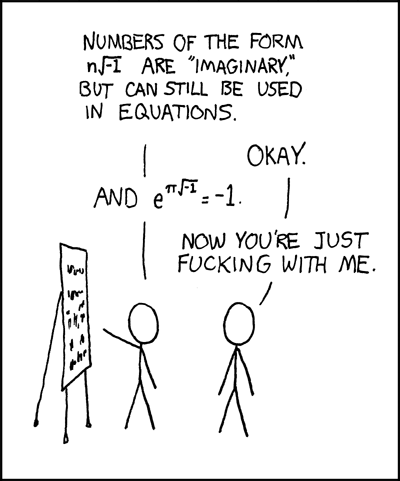
\includegraphics[width=9cm]{img/e_to_the_pi_times_i.png}}
\setlength{\parindent}{0em}
\parskip 1.5ex
\author{Matematik A}
\date{Vibenshus Gymnasium}
\title{Komplekse tal\\\medskip
\large Supplerende stof}
\hypersetup{
 pdfauthor={Matematik A},
 pdftitle={Komplekse tal},
 pdfkeywords={},
 pdfsubject={},
 pdfcreator={Emacs 27.2 (Org mode 9.4.4)}, 
 pdflang={Danish}}
\begin{document}

\maketitle
\tableofcontents

\begin{abstract}
Dette kompendium omhandler komplekse tal. Det er stærkt inspireret af / frit oversat fra \emph{Mathematical Methods for Physics and Engineering}, Second Edition, K.F. Riley, M.P. Hobson og S.J. Bence.
\end{abstract}

\section{Behovet for komplekse tal}
\label{sec:org593cd34}

Komplekse tal bruges i mange grene af matematikken (dog ikke umiddelbart i gymnasiet), men de opstår som udgangspunkt ved løsning af polynomiske ligninger. Som eksempel undersøges en specifik andengradsligning.

Betragt andengradsligningen

\begin{equation}
\label{andengrad}
    z^2 -4 z +5 = 0 
\end{equation}

Denne andengradsligning løses på sædvanlig vis

\begin{align}
\label{kompleks}
    z_{1,2} &= \frac{-b \pm \sqrt{b^2 - 4 \cdot a \cdot c}}{2 a} \nonumber\\
    z_{1,2} &= \frac{4 \pm \sqrt{\left(-4\right)^2 - 4 \cdot 1 \cdot 5}}{2 \cdot 1} \nonumber\\
    z_{1,2} &= 2 \pm \frac{\sqrt{-4}}{2} \,.
\end{align}

Begge løsninger indeholder kvadratroden af negative tal, hvilket ikke kan løses ved hjælp af de reelle tal. Det er dog ikke sandt at sige, at der ingen løsninger er til andengradsligningen. \emph{Algebraens fundamentalsætning} siger, at en andengradsligning altid vil have to løsninger. Disse to er faktisk givet ved ligning (\ref{kompleks}). Det andet led på højre side af ligning \eqref{kompleks} kaldes et \emph{imaginært} led, da det indeholder kvadratroden af et negativt tal. Det første led kaldes et \emph{reelt} led. Den fulde løsning er summen af et reelt led og et imaginært led. Denne løsning kaldes et \emph{komplekst} tal. Et plot af ligning (\ref{andengrad}) som et andengradspolynomium \(f(z)=z^2-4 z +5\) kan ses på figur \ref{fz}. Det kan ses, at \(f(z)\) ikke skærer \(z\)​-aksen, hvilket svarer til, at ligningen \(f(z)=0\) ingen rene reelle løsninger har.

\begin{figure}[htbp]
\centering
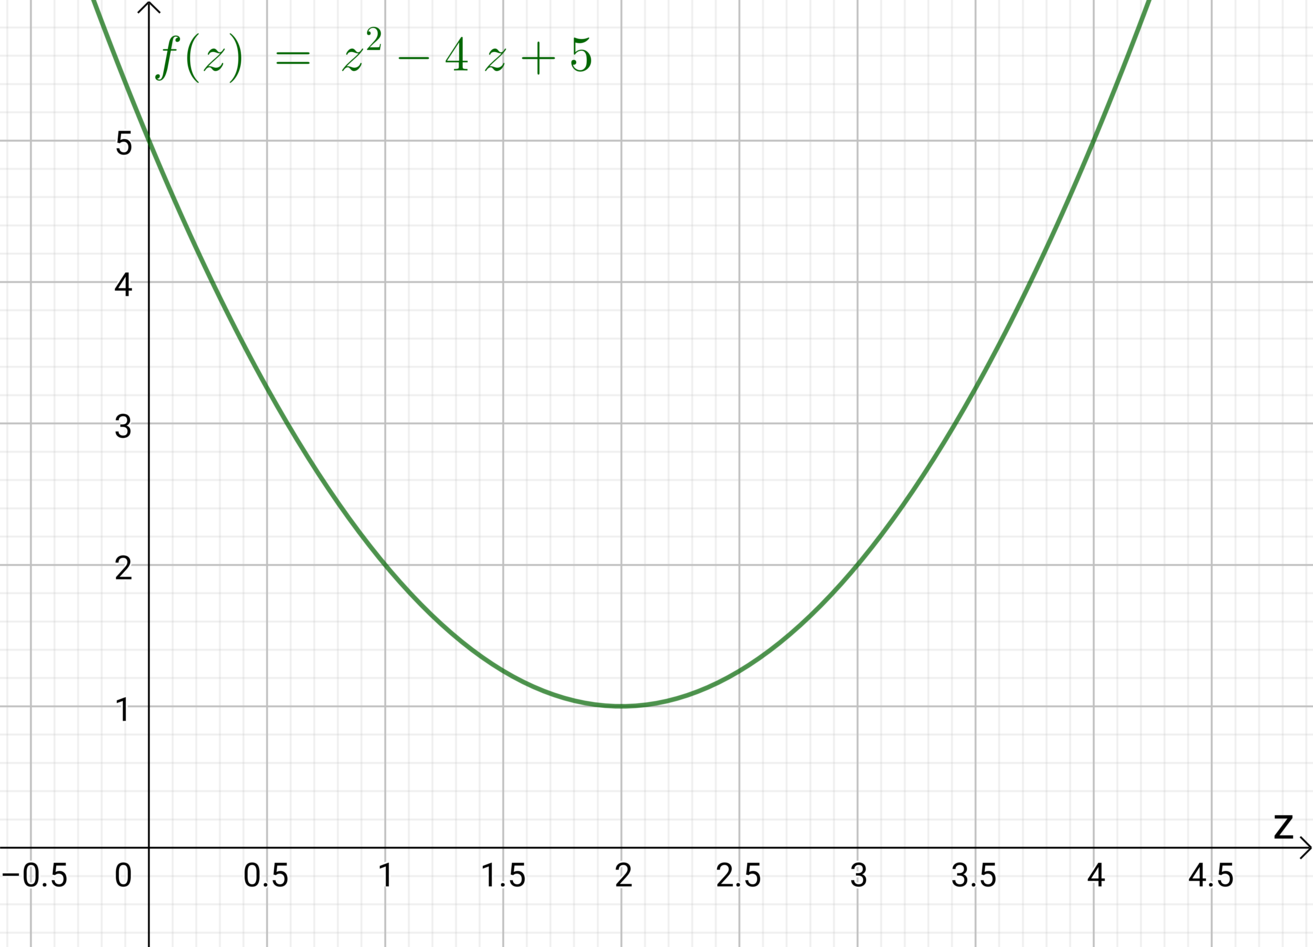
\includegraphics[width=.9\linewidth]{./img/fz_small.png}
\caption{\label{fz}Funktionen \(f(z) = z^2 -4z +5\).}
\end{figure}


Symbolet \(z\) er ikke valgt tilfældigt. Det er konventionen at repræsentere komplekse tal ved netop \(z\), hvor \(z\) er summen af en reel del \(x\) og \(i\) multipliceret med en imaginær del \(y\), udtrykt på følgende måde

$$z=x+i y \, ,$$

hvori \(i\)\footnote{Det skal nævnes, at nogle fysikere og særligt ingeniører bruger \(j\) i stedet for \(i\).} betegner kvadratroden af \(-1\), altså \(i=\sqrt{-1}\). Den reelle del \(x\) og den imaginære del \(y\) betegnes typisk henholdsvis ved \(Re(z)\) og \(Im(z)\). 

I dette specifikke eksempel gælder at \(\sqrt{-4} =2 \sqrt{-1} = 2 i\), hvorved de to løsninger til ligning (\ref{andengrad}) kan skrives som

$$z_{1,2} = 2 \pm \frac{2 i}{2} = 2 \pm i\,.$$

Af dette kan det ses, at \(x=2\) og \(y=\pm 1\).

For at kunne skrive komplekse tal mere kompakt op, bruges sommetider notationsformen

$$z = (x,y) \,,$$

hvor \(z\)'s komponenter kan betragtes som koordinater i et \(xy\)​-plot. Et sådant plot kaldes et \emph{Argand-diagram} og er en gængs repræsentation af komplekse tal. Et eksempel på et Argand-diagram kan ses på figur \ref{argand}. Argand-diagrammet kaldes undertiden også for det \emph{komplekse talplan}.

\begin{figure}[htbp]
\centering
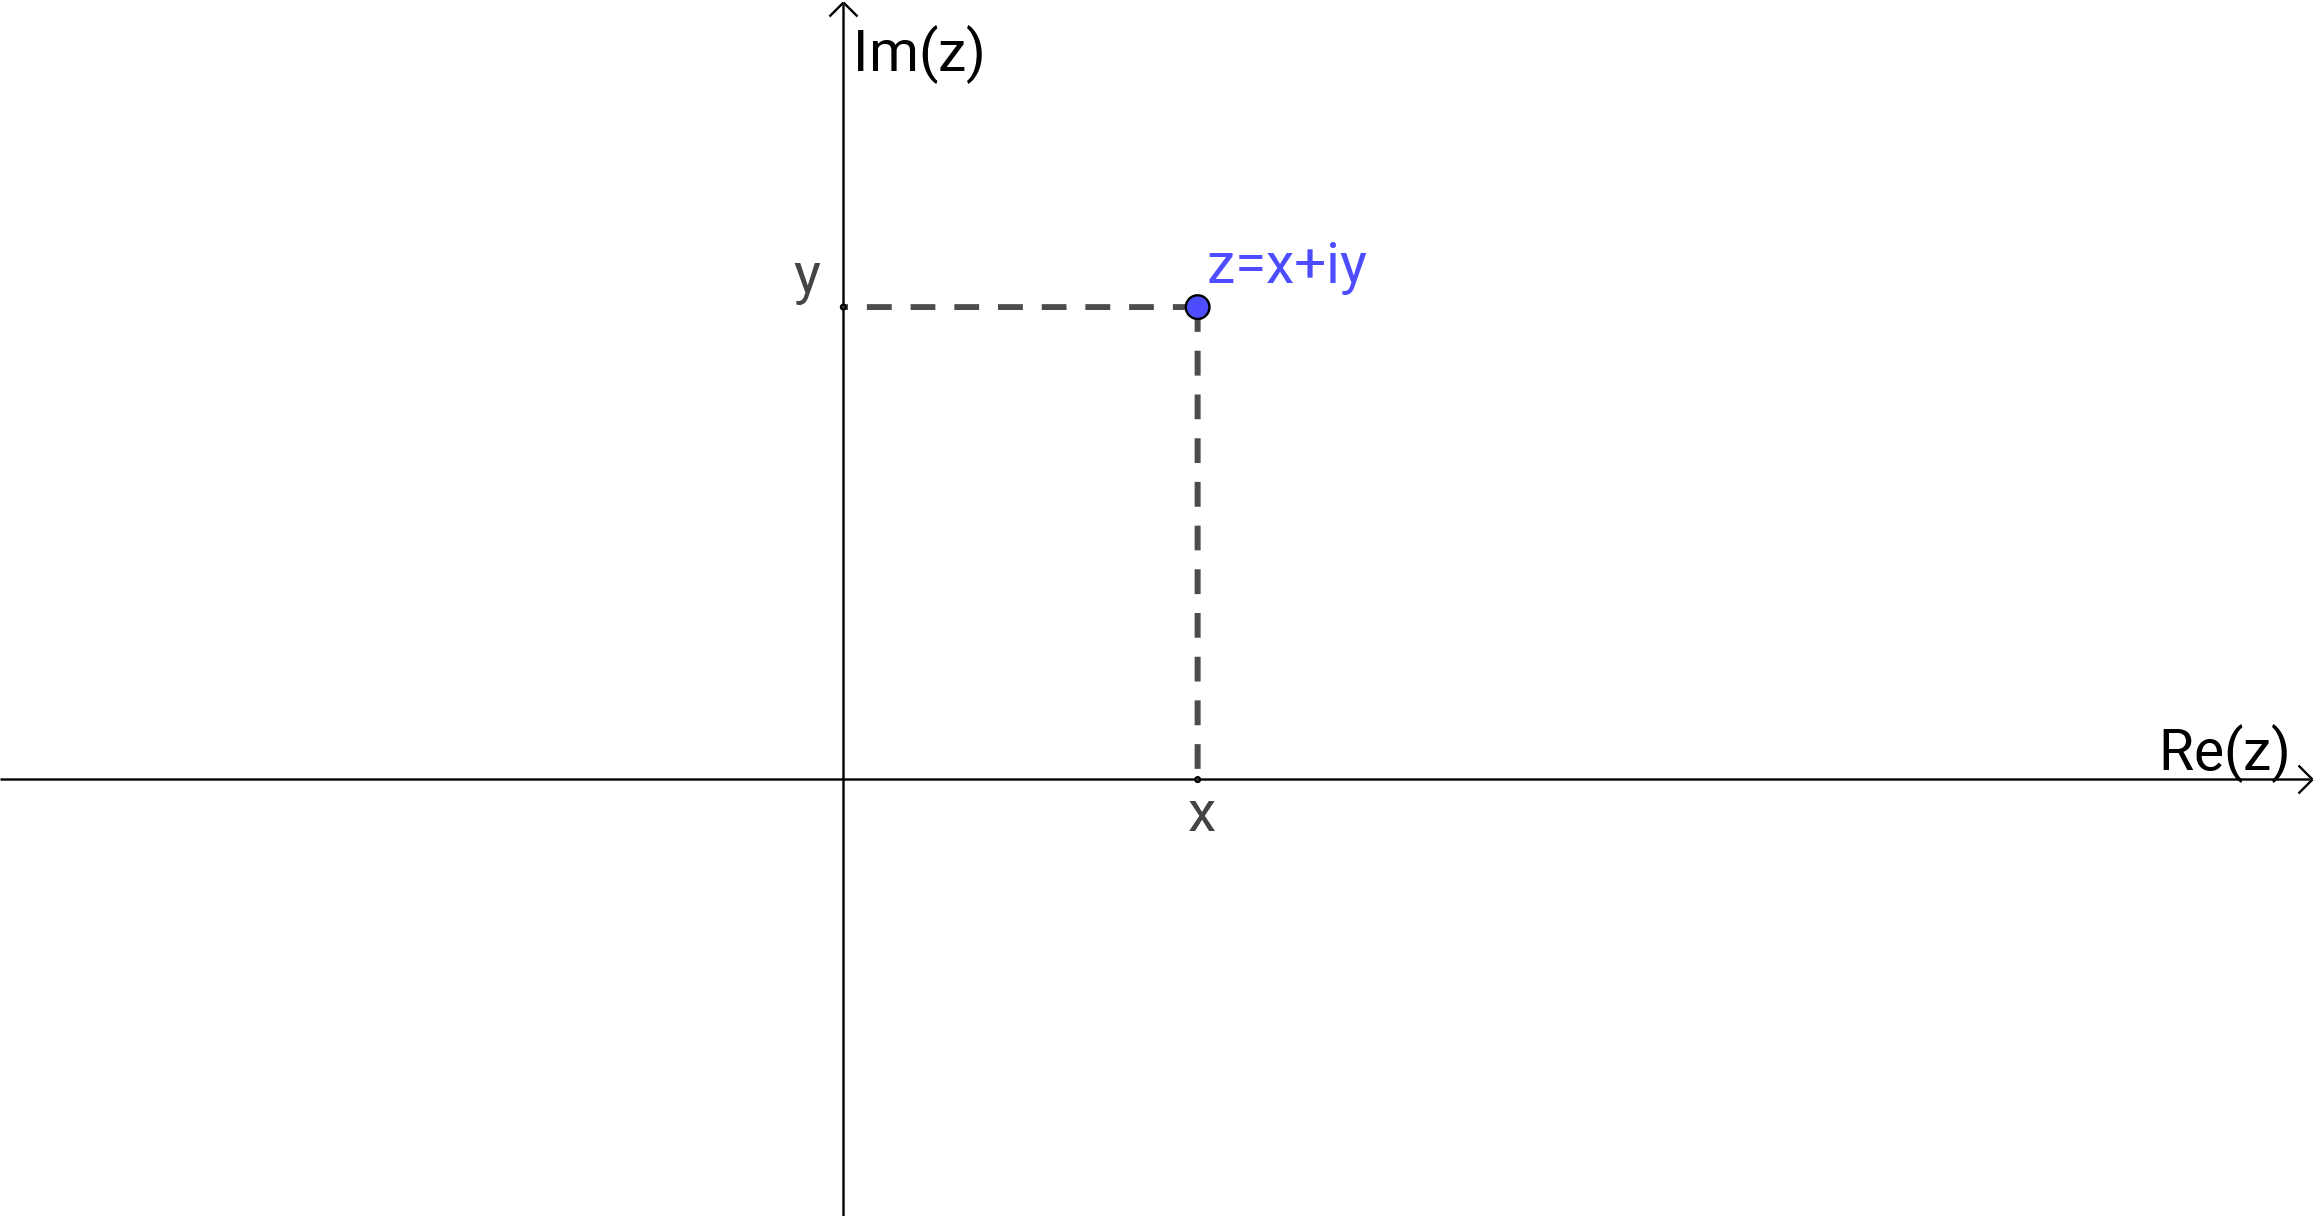
\includegraphics[width=.9\linewidth]{./img/argand.png}
\caption{\label{argand}Et eksempel på et Argand-diagram.}
\end{figure}

Eksemplet med løsningen af en andengradsligning kan generaliseres til løsning af andre polynomier med ordeiner større end 2, f.eks. 3., 4. osv. For et generelt \(n\)​'te-gradspolynomium \(f(z)\) gælder det, at der er præcis \(n\) løsninger til ligningen \(f(z)=0\).

Resten af dette kompendium vil uddybe komplekse tals algebra, deres polære repræsentation, komplekse eksponential- og logaritmefunktioner, bestemmelse af rødderne i polynomiske ligninger samt anvendelse af komplekse tal i forbindelse med differential- og integralregning.

\section{Manipulation af komplekse tal}
\label{sec:orgc97a2a8}

Dette afsnit omhandler de basale regneoperationer for komplekse tal. Der vil være visse ligheder med vektorregning.

\subsection{Addition og subtraktion}
\label{sec:orgdbd083b}

Generelt giver addition af to komplekse tal, \(z_1\) og \(z_2\), et andet komplekst tal. De reelle dele og imaginære dele adderes hver for sig på samme måde som for reelle tal.

$$z_1 + z_2 = (x_1 + i y_1) + (x_2 + i y_2) = (x_1 + x_2) + i ( y_1 + y_2) \, ,$$

Et Argand-diagram for addition af to komplekse tal kan ses på figur \ref{argand_addition}. Læg mærke til ligheden med addition af vektorer ved hjælp af et parallelogram.

\begin{figure}[htbp]
\centering
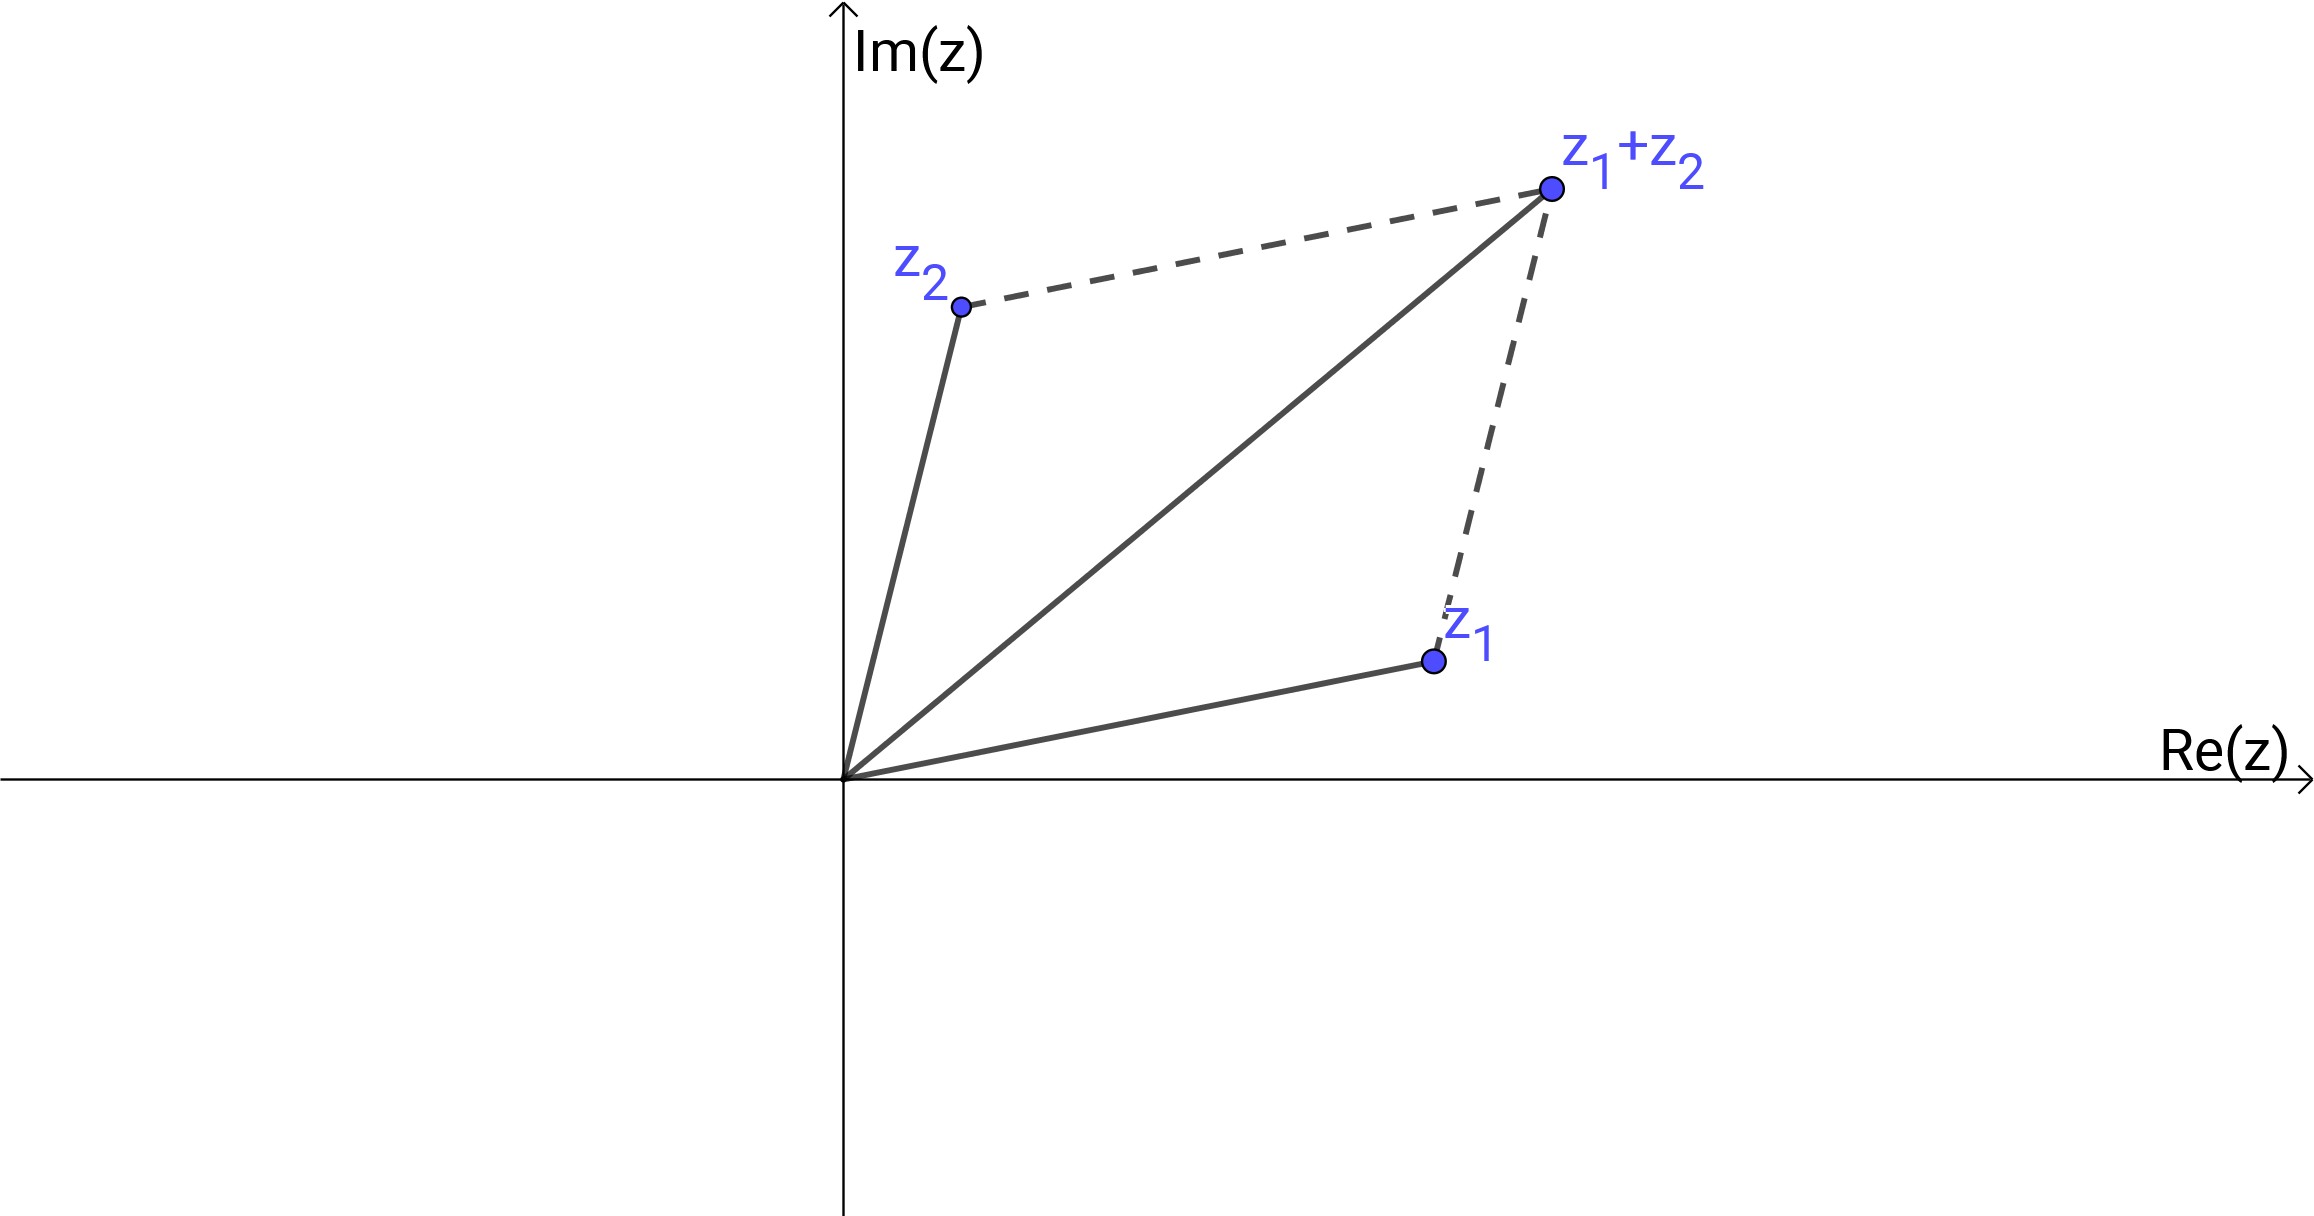
\includegraphics[width=.9\linewidth]{./img/argand_addition.png}
\caption{\label{argand_addition}Argand-diagrammet for addition af to komplekse tal. Læg mærke til ligheden med vektoraddition.}
\end{figure}

Yderligere skal det siges, at rækkefølgen for addition af komplekse tal er ligegyldig, da det gælder at

\begin{align*}
    z_1 + z_2 &= z_2 + z_1 & &\text{Kommutative lov}\\
    z_1 + (z_2 + z_3) &= (z_1 + z_2) + z_3 \,. & &\text{Associative lov}
\end{align*}

\subsubsection*{\textbf{Eksempel}}
\label{sec:org08da5c9}
\emph{Addition af de følgende komplekse tal}

\begin{itemize}
\item \(z_1 = 1 + 2i\)
\item \(z_2 = 3-4i\)
\item \(z_3 = -2 +i\)
\end{itemize}

Først adderes de reelle dele

$$x_1 + x_2 + x_3 = 1 + 3 - 2 = 2\,,$$

derefter addition af de imaginære dele

$$i y_1 + i y_2 + i y_3 = 2i - 4i + i = -i \,.$$

Alt i alt bliver summen af de tre komplekse tal følgende

$$z_1+z_2+z_3 = (1+2i) + (3-4i) + (-2+i) = 2 - i \quad \triangle$$

Subtraktion af komplekse tal foregår meget lig addition, hvor de reelle dele og imaginære dele subtraheres hver for sig. Lige som for reelle tal vil resultatet af subtraktion af to ens komplekse tal være nul.

\subsection{Modulus og argument}
\label{sec:orgc47fe78}

\emph{Modulus} for et komplekst tal \(z\) betegnes \(\lvert z \rvert\), og er defineret som

\begin{equation}
\label{modulus}
    \lvert z \rvert = \sqrt{x^2 + y^2} \, . 
\end{equation}

Modulus svarer til længden mellem det komplekse tals placering i det komplekse plan og origo. Sammenlignet med vektorregning svarer det til længden af en stedvektor.

\emph{Argumentet} af et komplekst tal benævnes \(arg(z)\), og er defineret som

\begin{equation}
\label{argument}
    arg(z) = \tan^{-1} \left(\frac{y}{x}\right) \,. 
\end{equation}

Modulus og argument er begge tegnet ind i Argand-diagrammet på figur \ref{modulus_og_argument}.

\begin{figure}[htbp]
\centering
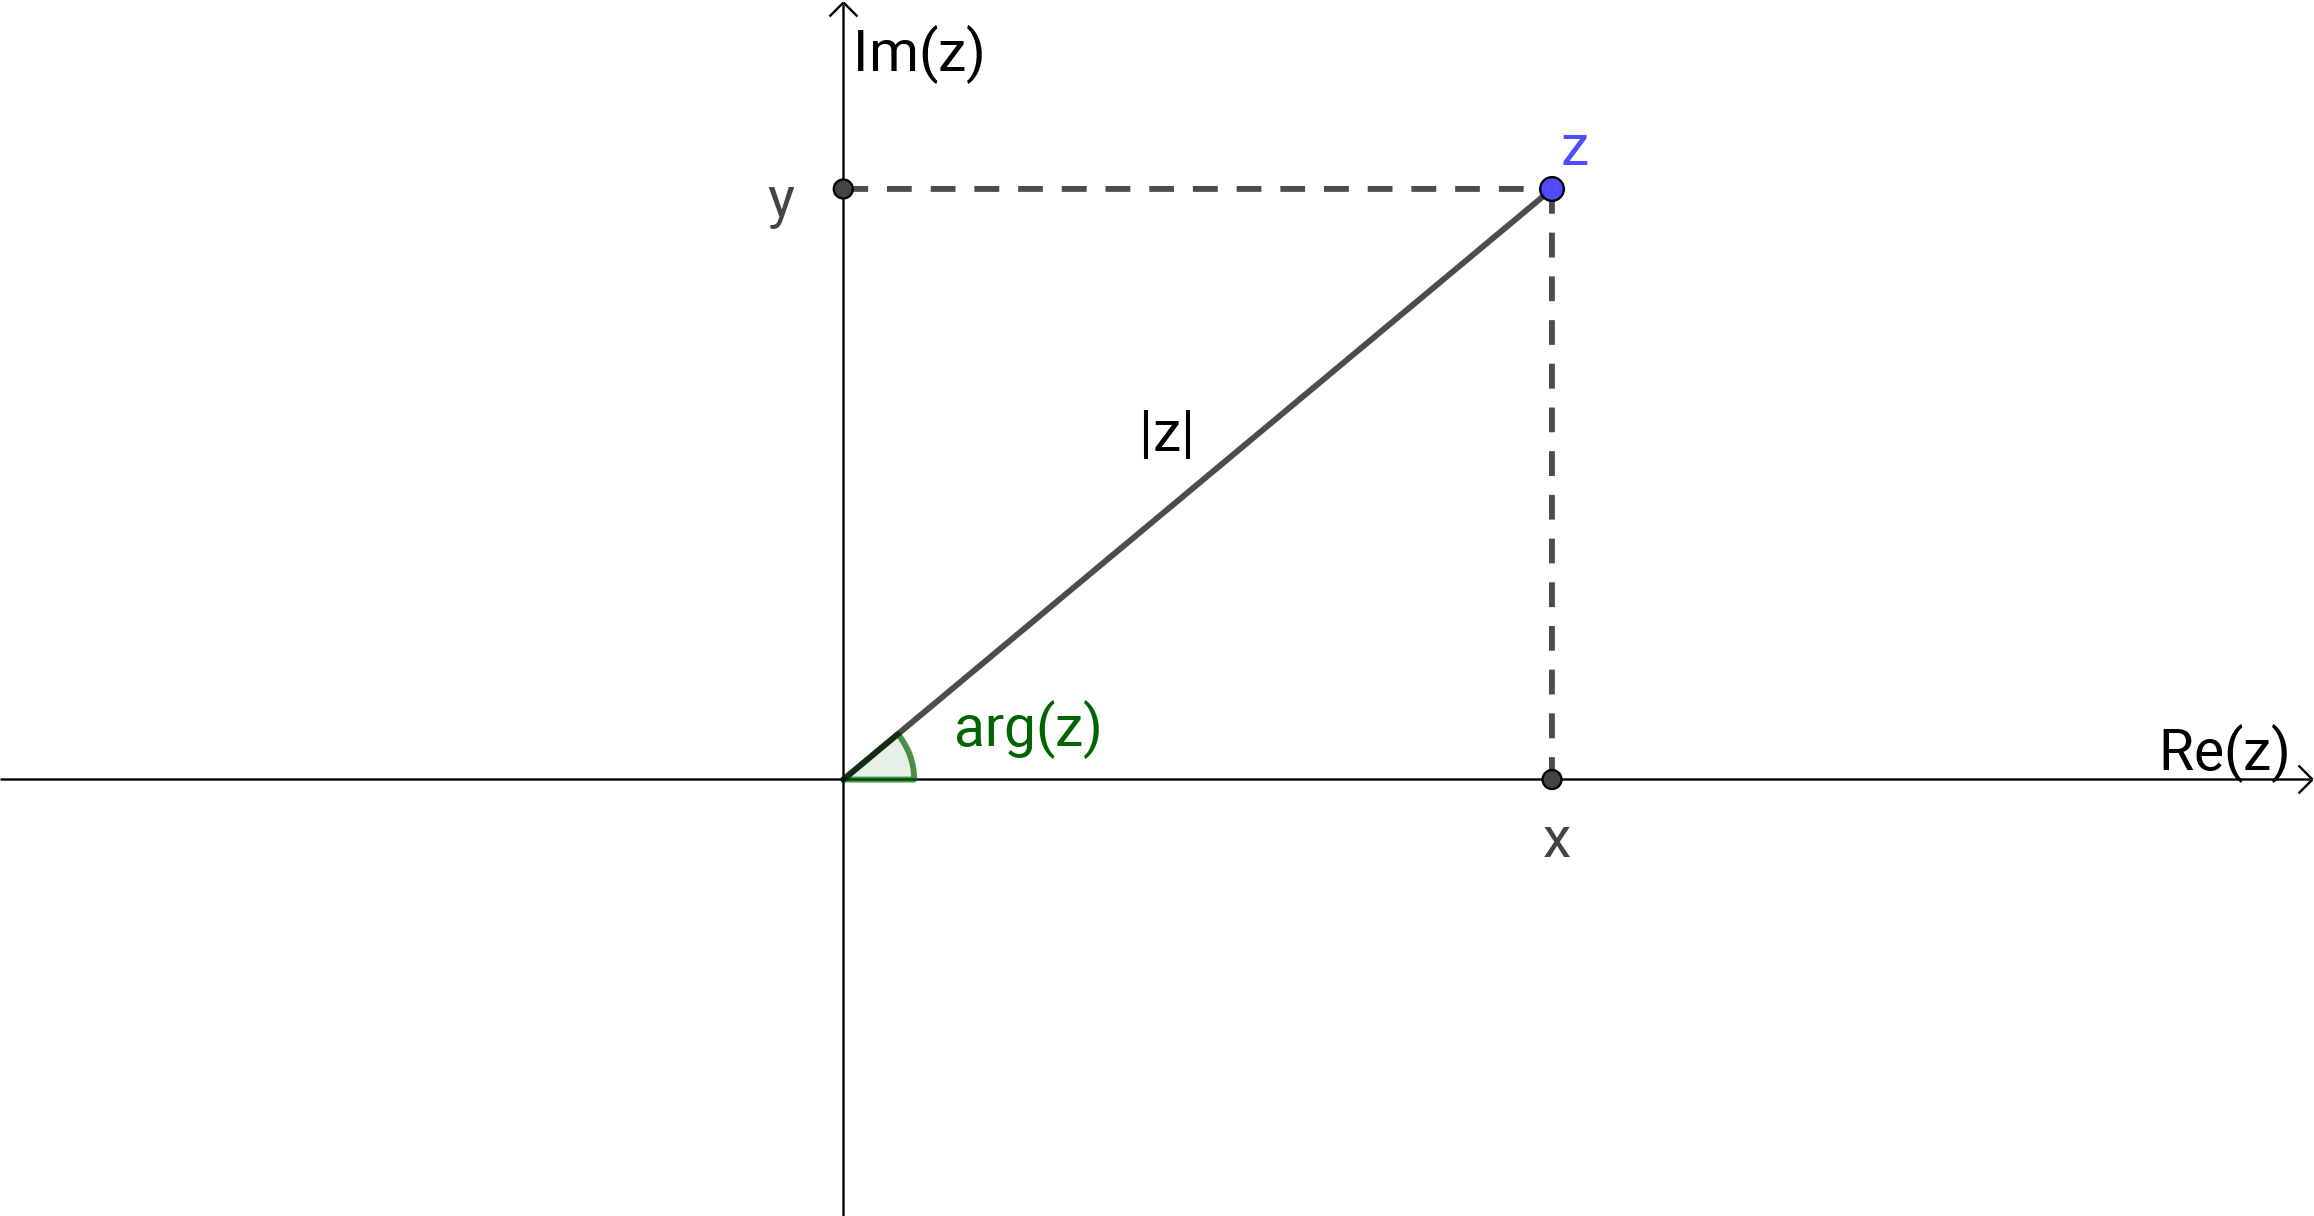
\includegraphics[width=.9\linewidth]{./img/modulus_og_argument.png}
\caption{\label{modulus_og_argument}Modulus og argument for et komplekst tal indtegnet i et Arganddiagram.}
\end{figure}

Det kan ses, at argumentet af \(z\) er vinklen mellem den positive reelle akse og linjen som forbinder origo og det komplekse tal. Vinklen måles i positiv omløbsretning, altså imod urets retning. Når argumentet af \(z\) skal beregnes skal man lægge særligt mærke til fortegnene for både \(x\) og \(y\), for at kunne afgøre, i hvilken kvadrant \(arg(z)\) er beliggende. Hvis f.eks. både \(x\) og \(y\) er negative, vil \(arg(z)\) ligge i intervallet \(-\pi < arg(z) < -\frac{\pi}{2}\) (tredje kvadrant) i stedet for i første kvadrant, som er i intervallet \(0 < arg(z) < \frac{\pi}{2}\). Denne information vil går ellers tabt, når forholdet mellem \(y\) og \(x\) bestemmes.

\subsubsection*{\emph{Eksempel}}
\label{sec:orgff3aa0b}
\emph{Find modulus og argument af det komplekse tal \(z=2-3i\).}

Først benyttes ligning (\ref{modulus}) til at bestemme modulus.

$$|z| = \sqrt{x^2+y^2} = \sqrt{2^2+(-3)^2} = \sqrt{13} \,.$$

Argumentet af \(z\) bestemmes vha. ligning (\ref{argument}).

$$arg(z) = \tan^{-1}\left(\frac{y}{x}\right) =\tan^{-1}\left(\frac{-3}{2}\right) =-0.9828 \,.$$

Dette stemmer overens med at \(z\) er beliggende i 4. kvadrant \(\triangle\).

\subsection{Multiplikation}
\label{sec:org0461aca}

Komplekse tal kan multipliceres med hinanden, hvilket generelt resulterer i endnu et komplekst tal. Produktet af to komplekse tal \(z_1\) og \(z_2\) bestemmes ved at multiplicere dem fuldt ud og huske på at \(i^2 = -1\). Dette er vist i det efterfølgende:

\begin{align*}
    z_1 \cdot z_2 &= (x_1 + i y_1) \cdot (x_2 + i y_2) \\
                  &= x_1 x _2 + i x_1 y_2 + i y_1 x_2 + i^2 y_1 y_2 \\
                  &= (x_1 x_2 - y_1 y_2) + i (x_1 y_2 + y_1 x_2) \, .
\end{align*}

\subsubsection*{\emph{Eksempel}}
\label{sec:orgf149bc4}
\emph{Multiplicer de komplekse tal \(z_1=3 + 2i\) og \(z_2 = -1 -4i\).}

Direkte multiplikation giver

\begin{align*}
    z_1 \cdot z_2 &= (3+2i) \cdot (-1 -4i) \\
                  &= -3 -2i - 12i -8 i^2 \\
                  &= 5-14i \quad \triangle
\end{align*}

Multiplikation af komplekse tal er både kommutativ og associativ, hvilket betyder, at rækkefølgen af de to faktorer er lige gyldig, samt at rækkefølgen af multiplikation af flere end to komplekse tal også er lige gyldig. Dette illustreres ved

\begin{align}
    z_1 \cdot z_2 &= z_2 \cdot z_1 & &\text{Kommutativ lov}\\
    (z_1 \cdot z_2)\cdot z_3 &= z_1 \cdot (z_2\cdot z_3) & &\text{Associativ lov} 
\end{align}

Produktet af to komplekse tal har yderligere følgende simple sammenhænge

\begin{align}
    |z_1\cdot z_2| &= |z_1| \cdot |z_2|  \label{modu} \\
    arg(z_1 \cdot z_2) &= arg(z_1) + arg(z_2) \,. \label{argu}
\end{align}

Begge sammenhænge vil blive udledt senere i kompendiet.

\subsubsection*{\emph{Eksempel}}
\label{sec:org53e06fe}
\emph{Eftervis at ligning \eqref{modu} gælder for de komplekse tal \(z_1=3+2i\) og \(z_2 = -1 -4i\), altså de samme komplekse tal, som i forrige eksempel.}

Fra forrige eksempel har vi

$$z_1 \cdot z_2 = 5-14i$$

Modulus af denne størrelse er

$$|z_1 \cdot z_2 |= |5-14i| = \sqrt{5^2 +(-14)^2} = \sqrt{221}\,.$$

Modulus for hver af de komplekse tal er

\begin{align*}
    |z_1| &= \sqrt{3^2+2^2} = \sqrt{13} \\
    |z_2| &= \sqrt{(-1)^2+(-4)^2} = \sqrt{17}
\end{align*}

Dette giver da

$$|z_1| \cdot |z_2| = \sqrt{13} \cdot \sqrt{17} = \sqrt{13 \cdot 17} = \sqrt{221} = |z_1 \cdot z_2|\,.$$

Hermed er ligning \eqref{modu} eftervist for de netop valgte komplekse tal. \(\triangle\)

Nu undersøges effekten af at multiplicere et komplekst tal med henholdsvis \(\pm 1\) og \(\pm i\). Disse fire multiplikatorer har alle modulus på 1. Fra ligning \eqref{modu} kan det ses, at et komplekst tal, \(z\), multipliceret med en af disse fire multiplikatorer giver et produkt, som har samme modulus som \(z\). Yderligere kan det ses af ligning \eqref{argu}, at argumentet for multiplikation af \(z\) med en af de fire nævnte multiplikatorer vil give summen af argumenterne hver for sig. Det kan da nu ses, at

\begin{itemize}
\item \(1 \cdot z= z\) : \(z\) forbliver uændret ved multiplikation med \(1\).

\item \(-1 \cdot z\) : Modulus forbliver uændret, mens argumentet ændres med vinklen \(\pi\). Dette svarer til at \(z\) roteres en halv omgang omkring origo i Argand-diagrammet.

\item \(i \cdot z\) : \(z\) roteres \(\frac{\pi}{2}\) omkring origo. Altså en kvart omgang i positiv omløbsretning.

\item \(-i \cdot z\) : \(z\) roteres \(-\frac{\pi}{2}\) omkring origo. Altså en kvart omgang i negativ omløbsretning.
\end{itemize}

Disse geometriske fortolkninger af multiplikation med de fire multiplikatorer 1, -1, \(i\) og \(-i\) kan ses på figur \ref{multiplikation}.

\begin{figure}[htbp]
\centering
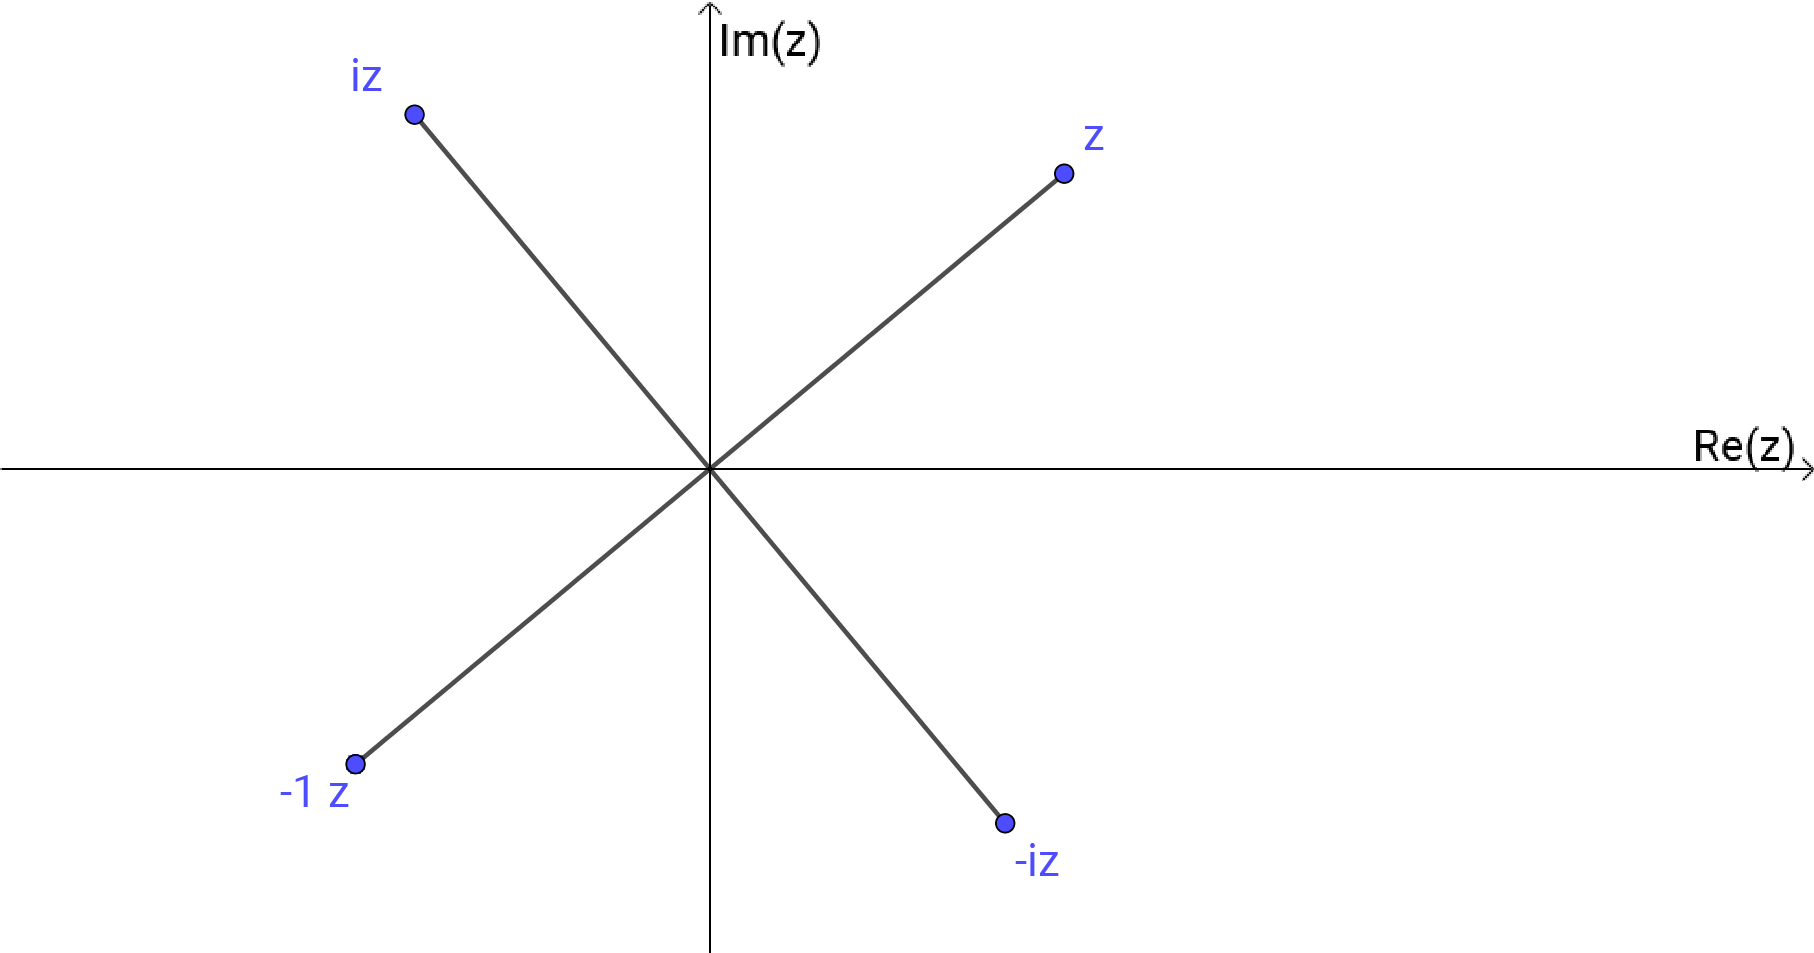
\includegraphics[width=.9\linewidth]{./img/multiplikation.png}
\caption{\label{multiplikation}Multiplikation af et komplekst tal og \(\pm 1\) samt \(\pm i\).}
\end{figure}

\subsubsection*{\emph{Eksempel}}
\label{sec:org19a00ff}
\emph{Benyt den geometriske fortolkning af multiplikation med \(i\) til at bestemme produktet \(i \cdot (1-i)\).}

\(1-i\) har argumentet 

$$arg(1-i) = \tan^{-1}\left( \frac{-1}{1}\right) = -\frac{\pi}{4}$$

og modulus

$$|1-i| = \sqrt{1^2+(-1)^2} = \sqrt{2}\,.$$

\(1-i\) ligger altså i 4. kvadrant svarende til \(45^\circ\) under den reelle akse. Ved at multiplicere med \(i\) forbliver modulus på \(\sqrt{2}\), mens argumentet drejes \(\frac{\pi}{2}\) i positiv omløbsretning, hvilket resulterer i et argument på \(+\frac{\pi}{4}\). Det komplekse tal med dette modulus og argument er \(1+i\), hvilket vil sige, at

$$i\cdot(1-i) = 1+i\,.$$

Dette kan simpelt verificeres ved direkte multiplikation

$$i\cdot(1-i) = i - i^2 = i - (-1) = 1 +i \,. \quad \triangle$$

Division af to komplekse tal foregår på tilsvarende vis som for multiplikation, men kræver kendskab til begrebet \emph{kompleks konjugation}, hvilket derfor vil blive introduceret først.

\subsection{Kompleks konjugation}
\label{sec:org7b5e2b2}

For det komplekse tal \(z=x+iy\) findes det \textbf{kompleks konjugerede} tal \(z^*\) ved simpelt at ændre fortegnet på den imaginære del af \(z\). Det vil sige for

\begin{align*}
    z&=x+iy \to \\
    z^*&=x-iy \,.
\end{align*}

Mere generelt kan det kompleks konjugerede tal til \(z\) defineres som det (komplekse) tal, der har samme modulus som \(z\) selv, og som ved multiplikation med \(z\) resulterer i et reelt tal. Det vil sige, at der ingen imaginær del er i produktet \(z \cdot z^*\).

I det tilfælde hvor \(z\) kan skrives som \(z=x+iy\), kan det let verificeres, at \(z \cdot z^*\) giver et reelt resultat:

$$z \cdot z^* = (x+iy) \cdot (x-iy) = x^2 -ixy +ixy -i^2 y^2 = x^2 -i^2 y^2 = x^2 -(-1) y^2 = x^2+y^2 = |z|^2 \,.$$

Den geometriske fortolkning af kompleks konjugation svarer til at \emph{spejle} \(z\) i den reelle akse i Argand-diagrammet. Dette kan ses på figur \ref{fig:konjugation}.

\begin{figure}[htbp]
\centering
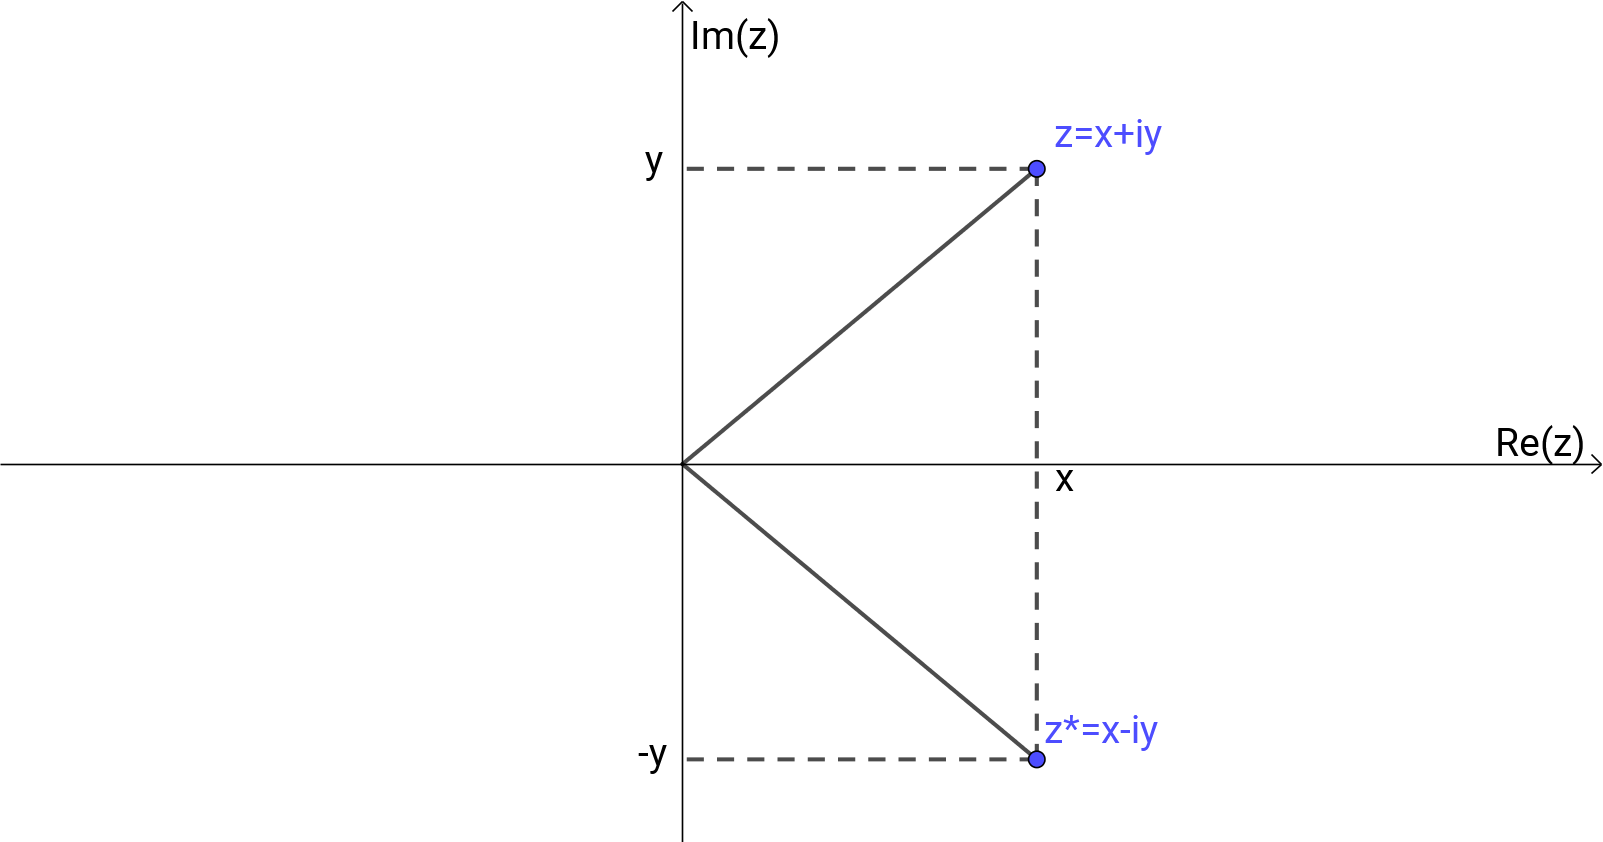
\includegraphics[width=.9\linewidth]{./img/konjugation.png}
\caption{\label{fig:konjugation}Den geometriske fortolkning af kompleks konjugation, som en spejling i den reelle akse.}
\end{figure}

\subsubsection*{\emph{Eksempel}}
\label{sec:orga92199f}
\emph{Find den kompleks konjugerede til \(z=a+2i+3ib\).}

Det komplekse tal kan omskrives til

$$z= a +i\cdot(2+3b) \,.$$

Nu skal \(i\) erstattes af \(-i\) for at finde den kompleks konjugerede

$$z^*= a -i\cdot(2+3b) \,.\quad \triangle$$

I nogle tilfælde er det ikke altid let at skrive udtrykket for \(z\) om til standardformen \(x+iy\). For to komplekse tal \(z_1\) og \(z_2\) er det dog let at vise, at den kompleks konjugerede af deres sum eller differens er lig summen eller differencen af deres individuelle kompleks konjugerede. De samme egenskaber gør sig gældende for henholdsvis produkter og kvotienter mellem to komplekse tal. Matematisk kan dette skrives op som

\begin{align*}
    (z_1 \pm z_2)^* &= z_1^* \pm z_2^* \\
    (z_1 \cdot z_2)^* &= z_1^* \cdot z_2^* \\
    \left(\frac{z_1}{z_2}\right)^* &= \frac{z_1^*}{z_2^*} \,.
\end{align*}

Ved at benytte disse regler er det muligt at bestemme den kompleks konjugerede til et vilkårligt kompliceret udtryk ved at udskifte alle \(i\)'er i udtrykket med \(-i\) og omvendt. Dette kræver dog, at alle imaginære dele er synlige i udtrykket.

\subsubsection*{\emph{Eksempel}}
\label{sec:org979f412}
\emph{Bestem den kompleks konjugerede til det komplekse tal \(z=w^{(3y+2ix)}\), hvor \(w=x+5i\).}

\(w\) selv indeholder både reelle og imaginære dele, hvilket skal skrives ud, for at finde den kompleks konjugerede for det samlede udtryk. Dette gøres først for derefter at skifte fortegnet for alle \(i\)'er:

\begin{align*}
    z &= w^{(3y+2ix)} \\
    z &= (x+5i)^{(3y+2ix)} \to \\
    z^* &= (x-5i)^{(3x-2ix)} \, . \quad \triangle
\end{align*}

Ud over de føromtalte regler for komplekse tal og deres konjugerede er her fem regler mere, som let kan eftervises. Hvis \(z=x+iy\), da gælder det at

\begin{align}
    \left(z^*\right)^* &= z \\
    z\cdot z^* &= |z|^2 \\
    z+ z^* &= 2 \cdot Re(z) = 2 x \\
    z-z^* &= 2i \cdot Im(z) = 2iy \\
    \frac{z}{z^*} &= \left(\frac{x^2-y^2}{x^2+y^2} \right) + i \left(\frac{2 x y}{x^2+y^2}\right) \label{kvotient}\,.
\end{align}

Udledningen af det sidste udtryk kræver kendskab til division af to komplekse tal, hvilket det næste afsnit netop omhandler.

\subsection{Division}
\label{sec:org7e7ebeb}

Division af to komplekse tal har visse ligheder med multiplikation. For de to komplekse tal \(z_1= x_1+y_1 i\), \(z_2=x_2+y_2 i\) er kvotienten mellem dem

\begin{equation}
    \frac{z_1}{z_2} = \frac{x_1+y_1 i}{x_2+y_2 i}
\end{equation}

Her er det svært at skelne den reelle og imaginære del fra hinanden. For at separere den reelle og komplekse del multipliceres både tæller og nævner med den oprindelige nævners kompleks konjugerede. Ud fra definitionen på kompleks konjugation vil dette give et reelt tal i nævneren. Dette giver nu

\begin{align*}
    \frac{z_1}{z_2} &= \frac{x_1+y_1 i}{x_2+y_2 i} \\
    \frac{z_1}{z_2} &= \frac{(x_1+y_1 i)\cdot(x_2-y_2 i)}{(x_2+y_2 i)\cdot(x_2-y_2 i)} \\
    \frac{z_1}{z_2} &= \frac{(x_1 x_2 + y_1 y_2)+i(x_2 y_1 - x_1 y_2)}{x_2^2+y_2^2} \\
    \frac{z_1}{z_2} &= \frac{x_1 x_2 + y_1 y_2}{x_2^2+y_2^2}+i\frac{x_2 y_1 - x_1 y_2}{x_2^2+y_2^2} 
\end{align*}

Det kan ses, at den reelle del og den imaginære del nu er adskilt.

I det tilfælde hvor \(z_2=z_1^*\), således at \(x_2=x_1\) og \(y_2=- y_1\), fås det generelle udtryk i ligning \eqref{kvotient}.

\subsubsection*{\emph{Eksempel}}
\label{sec:org500bf06}
\emph{Udtryk \(z\) på komponentformen, \(x+yi\), når \(z=\frac{3-2i}{-1+4i}\).}

Tæller og nævner multipliceres med den kompleks konjugerede til nævneren

\begin{align*}
    z &=\frac{3-2i}{-1+4i} \\
    z &=\frac{(3-2i)(-1-4i)}{(-1+4i)(-1-4i)} \\
    z &=\frac{-11 -10i}{17} \\
    z &=\frac{-11}{17} -\frac{10}{17}i \, . \quad \triangle
\end{align*}

Modulus og argument for kvotienten mellem to komplekse tal har samme egenskaber som produktet mellem dem, nemlig at følgende gælder

\begin{align}
    \left\lvert\frac{z_1}{z_2}\right\rvert &= \frac{\lvert z_1 \rvert}{\lvert z_2 \rvert} \\
    arg\left( \frac{z_1}{z_2} \right) &= arg(z_1) - arg(z_2) \,.
\end{align}

Disse udtryk vil blive bevist i et senere afsnit.

\subsection{Polær repræsentation af komplekse tal}
\label{sec:org9ae9365}

I nogle tilfælde er det lettest at betragte et komplekst tal som summen af en reel del og en imaginær del. I andre tilfælde viser det sig at være lettere at benytte den \emph{polære repræsentation}. Denne repræsentationsform gør brug af den komplekse eksponentialfunktion, som er defineret som\footnote{Skrevet som en sum er den givet ved \(e^z \equiv \sum_{j=0}^{\infty} \frac{z^j}{j!}\).}

\begin{equation}
\label{expz}
    e^z = exp(z) \equiv 1 + z + \frac{z^2}{2!} + \frac{z^3}{3!} + \cdots \, . 
\end{equation}

Ved at benytte de passende serier for \(e^{z_1}\) og \(e^{z_2}\) er det muligt at vise, at

\begin{equation}
\label{ee}
    e^{z_1} \cdot e^{z_2} = e^{z_1+z_2} \,,
\end{equation}

hvilket stemmer overens med eksponentialregnereglerne for reelle tal.

Nu betragtes eksponeringen af det rent imaginære tal \(z=i\theta\), hvor \(\theta\) selv er reelt

\begin{equation}
\label{taylor}
\begin{aligned}
    e^z = e^{i\theta}&= 1+ i\theta + \frac{(i \theta)^2}{2!} + \frac{(i\theta)^3}{3!} + \frac{(i\theta)^4}{4!}+ \frac{(i\theta)^5}{5!}+\cdots  \\
                     &= 1 + i\theta - \frac{\theta^2}{2!} - \frac{i\theta^3}{3!} + \frac{\theta^4}{4!} + \frac{i\theta^5}{5!} +\cdots \\
                     &=\left(1- \frac{\theta^2}{2!} + \frac{\theta^4}{4!} - \cdots\right) + i \left(\theta - \frac{\theta^3}{3!} + \frac{\theta^5}{5!}-\cdots \right) \\
                     &= \cos \left(\theta\right) + i \sin\left(\theta\right)\,,
\end{aligned} 
\end{equation}

hvor den sidste linje gør brug af \emph{Taylor-udviklingerne}​\footnote{Taylor-udvikling er et andet interessant emne, som kunne fylde et helt kompendium sig selv. I behøver ikke at bekymre jer yderligere om denne del.} for henholdsvis sinus og cosinus, der er givet ved

\begin{align*}
    \sin \left(\theta \right) &= \left(\theta - \frac{\theta^3}{3!} + \frac{\theta^5}{5!}-\cdots \right) \\
    \cos \left(\theta \right) &=\left(1- \frac{\theta^2}{2!} + \frac{\theta^4}{4!} - \cdots\right) \,.
\end{align*}

Udtrykket 

\begin{equation}
\label{euler}
    e^{i\theta} = \cos \left(\theta\right) + i \sin \left(\theta\right)
\end{equation}

er ganske særligt, og kaldes \emph{Eulers ligning}, efter dets opdager Leonhard Euler.

Fra Eulers ligning kan følgende lignende sammenhæng også opskrives

$$e^{i n \theta} = \cos \left(n \theta\right) + i \sin \left(n \theta\right)\,,$$

for alle \(n\).

\begin{figure}[htbp]
\centering
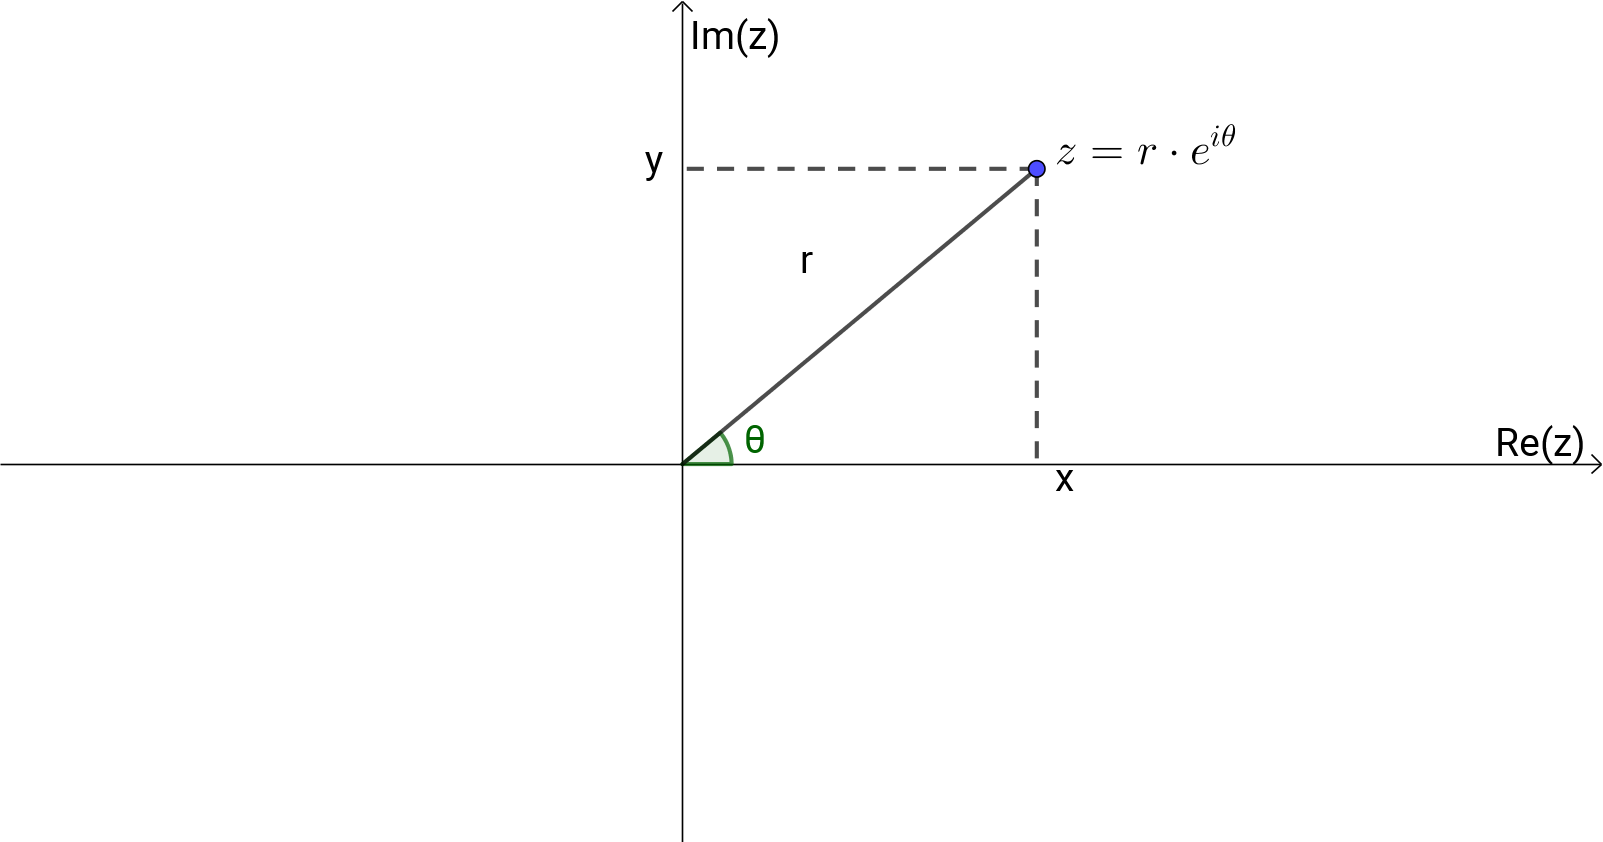
\includegraphics[width=.9\linewidth]{./img/euler.png}
\caption{\label{fig_euler}Den polære repræsentation af et komplekst tal.}
\end{figure}

Fra Eulers ligning (\ref{euler}) og figur \ref{fig_euler} er det muligt at udlede følgende sammenhæng

\begin{align*}
    r \cdot e^{i\theta} = r \left(\cos\left(\theta\right) + i \sin\left(\theta\right)\right)\\
    r \cdot e^{i\theta} = x + iy \,.
\end{align*}

Et komplekst tal kan af disse grunde skrives på  polær form, som

\begin{equation}
    z = r \cdot e^{i \theta}
\end{equation}

På figur \ref{fig_euler} kan \(r\) identificeres som \(|z|\) og \(\theta\) som \(arg(z)\). Denne simple repræsentation for modulus og argument for et komplekst tal er en af hovedgrundene for brugen af den polære notationsform. Vinklen \(\theta\) ligger konventionelt i intervallet \(-\pi < \theta \leq \pi\), men siden en rotation med \(\theta\) er det samme som en rotation med \(2 n \pi + \theta\), hvor \(n\) er et heltal, gælder

\begin{equation}
\label{flere_omgange_euler}
r \cdot e^{i \theta} = r \cdot e^{i(\theta+2 n \pi)} \,.
\end{equation}

Den algebra, som er tilknyttet den polære repræsentation af et komplekst tal (\(z=r \cdot e^{i\theta}\)), er forskellig for algebraen for komplekse tal repræsenteret ved henholdsvis en reel del og en imaginær del (\(z=x+iy\)). Beregningerne på den ene eller anden måde giver dog selvfølgelig det samme resultat. Nogle regneoperationer viser sig at være meget nemmere at udføre på polær form, mens andre er nemmere i komponentform (undertiden også kaldet rektangulær form). Den bedste repræsentationsform for et givent problem afhænger derfor af de krævede beregninger.

\subsection{Simple identiteter}
\label{sec:orga29aa0c}

Ud fra Eulers ligning (\ref{euler}) og ligning (\ref{flere_omgange_euler}) samt en figur af den komplekse enhedscirkel er det muligt at argumentere for følgende simple, men brugbare identiteter:

\begin{equation}
\label{simple_identiteter}
\begin{aligned}
1 &= e^{2 \pi k i} \\
i &= e^{\frac{\pi}{2}i + 2 \pi k i} = e^{\frac{\pi}{2}\left( 4k +1 \right)i}\\
-1 &= e^{\pi i + 2 \pi k i} = e^{\pi \left( 2k+1 \right)i}\\
-i &= e^{-\frac{\pi}{2}i+2\pi k i} = e^{\frac{\pi}{2}\left( 4k-1 \right)i}
\end{aligned}
\end{equation}

\begin{figure}[htbp]
\centering
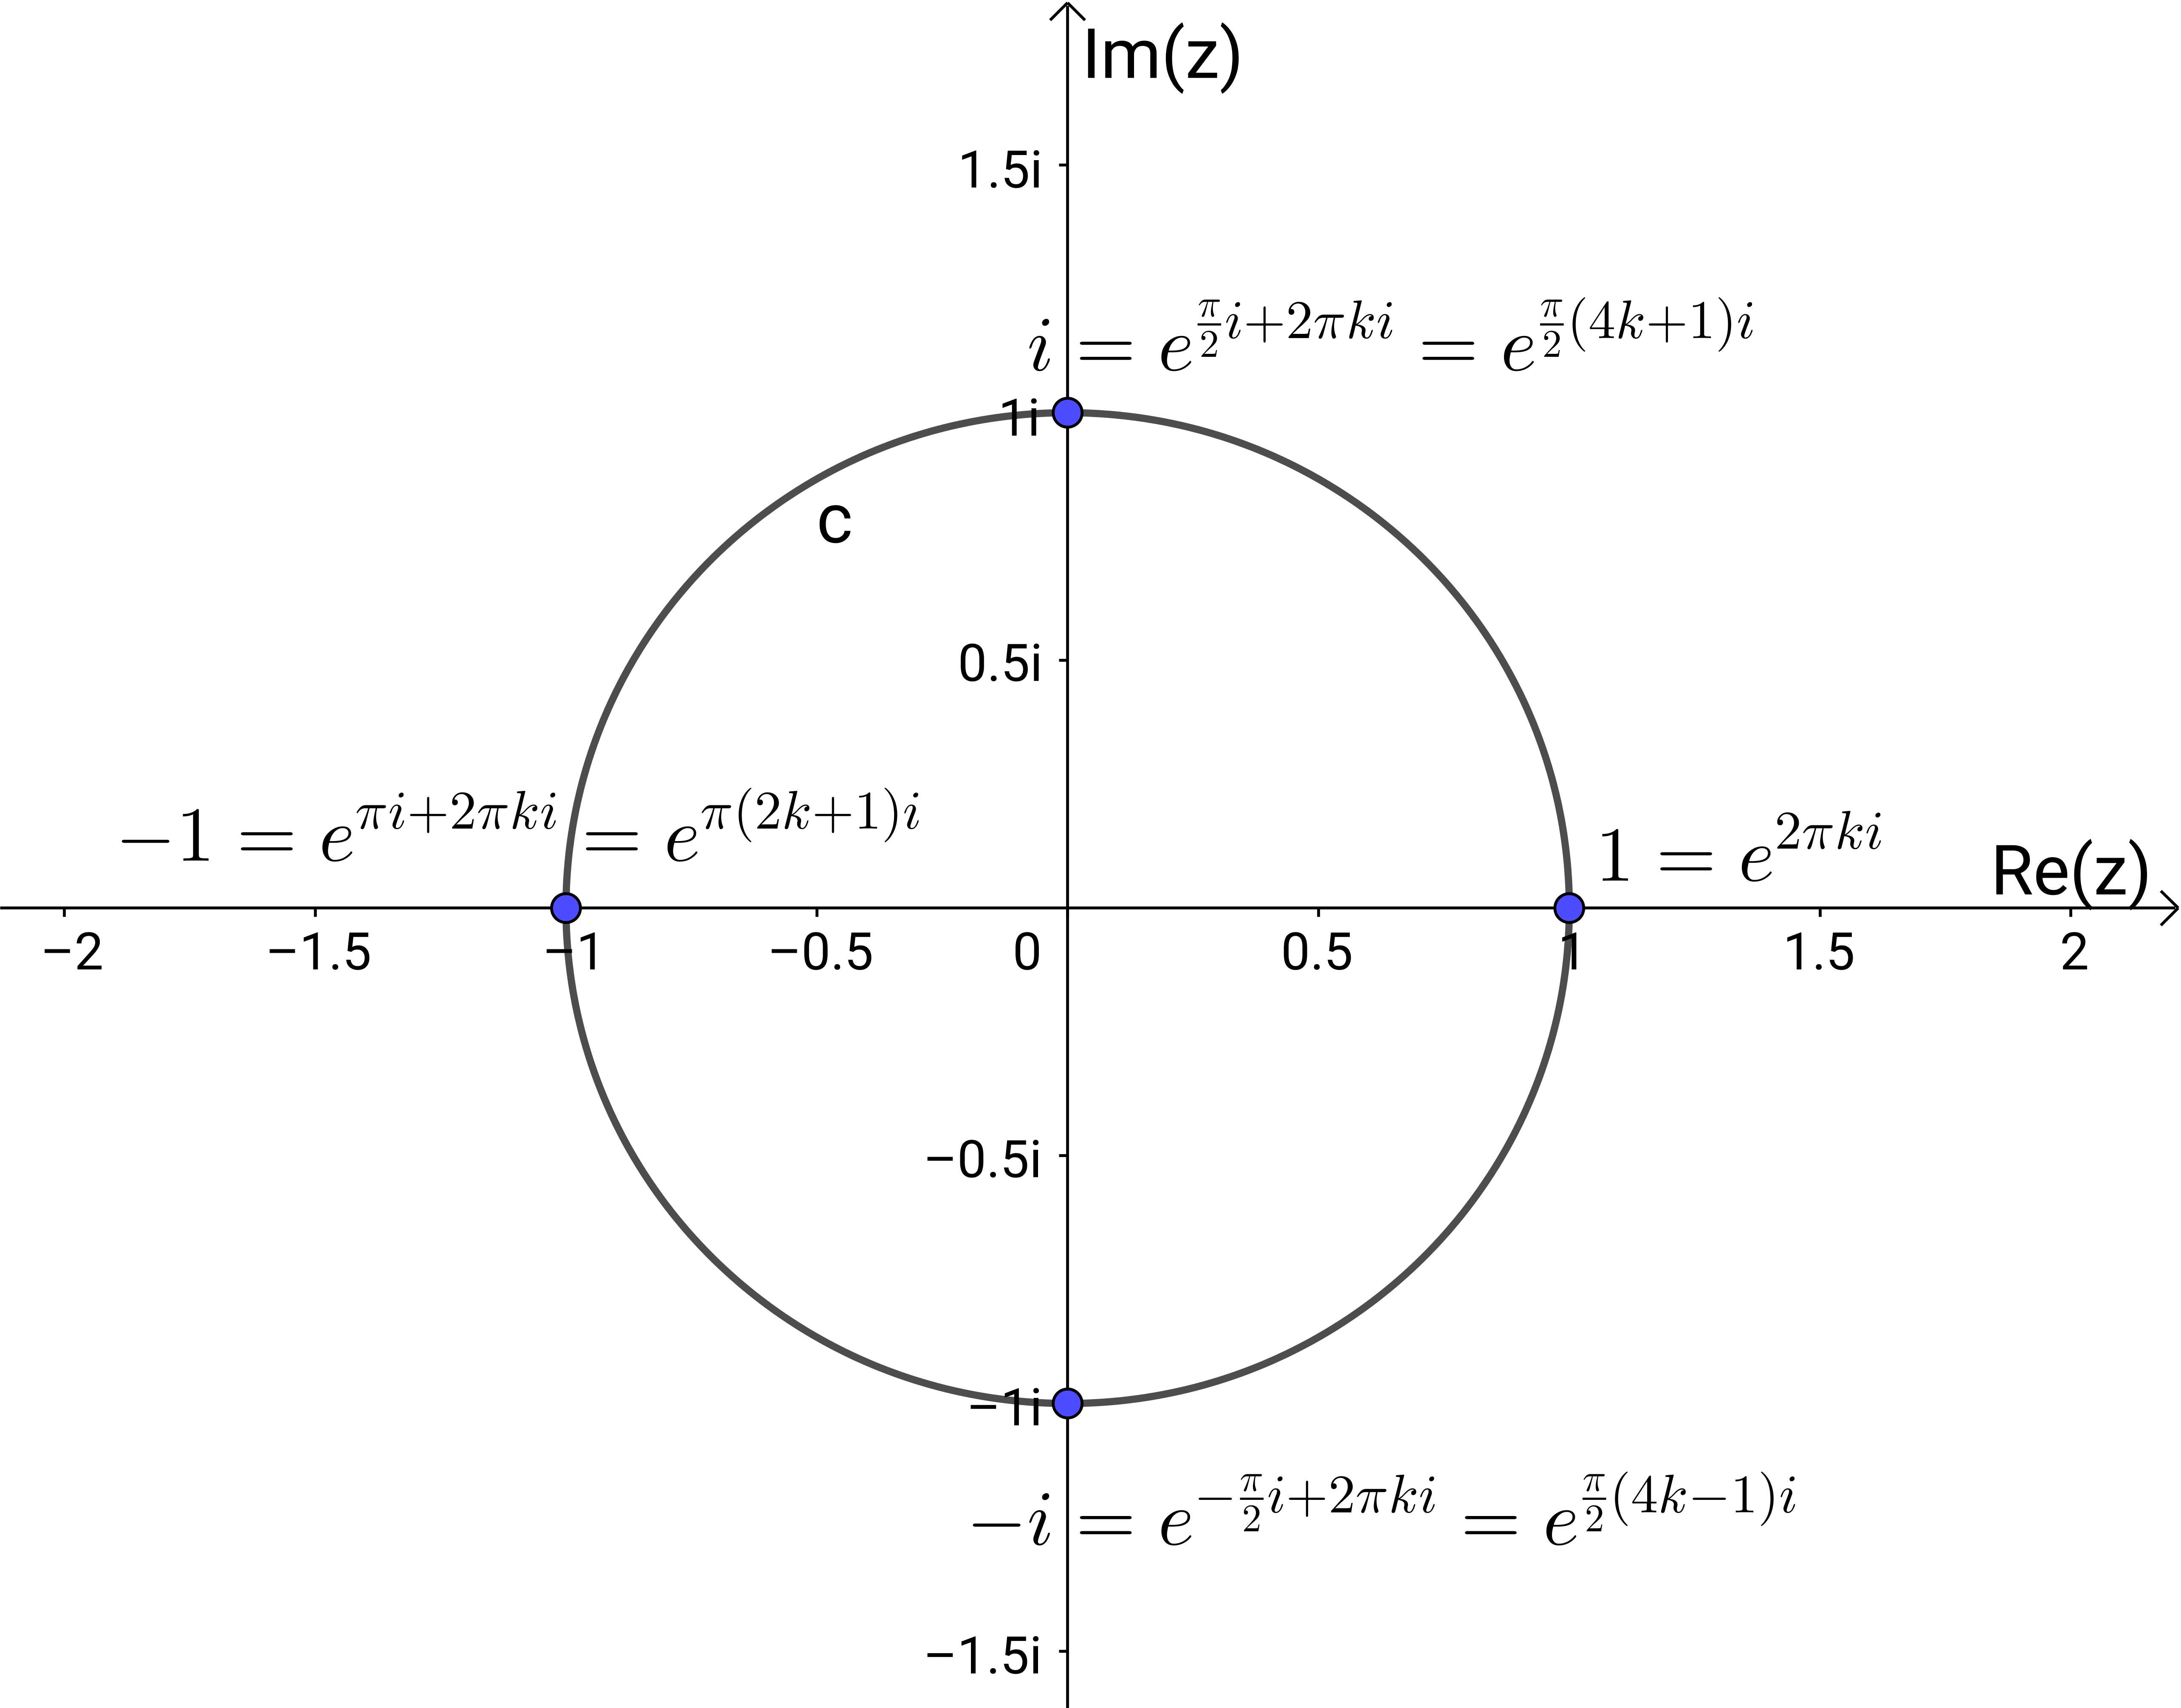
\includegraphics[width=10cm]{./img/kompleks_enhedscirkel_identiteter.png}
\caption{\label{fig:simple_identiteter}Den komplekse enhedscirkel med simple identiteter indsat.}
\end{figure}

Argumentationen for de førnævnte identiter tager udgangspunkt i figur \ref{fig:simple_identiteter}. \(1\) ligger på den reelle akse i afstanden 1 fra origo og dermed er argumentet (vinklen med den reelle akse) i første omgang blot lig nul, men ved hjælp af ligning (\ref{flere_omgange_euler}) kan det ses, at der kan lægges et helt antal omgange oveni, hvilket er repræsenteret af \(2\pi k\). Det samme princip gør sig gældende for de tre resterende identiteter. \(i\) ligger op ad den imaginære akse, og har altså et argument på \(\frac{\pi}{2}\). Oven i det lægges der et helt antal omgange. \(-1\) har i første omgang et argument på \(- \pi\), hvor der igen lægges et helt antal omgange oveni. Endelig kan argumentet til \(-i\) repræsenteres som \(\frac{3}{2}\pi\) eller endnu nemmere som \(- \frac{\pi}{2}\pi\). Her anvendes sidstnævnte repræsentation, da det giver symmetri i identiteterne, og hvem kan ikke godt lide symmetrier. De nævnte identiteter kan være meget anvendelige i f.eks. opgave 3, som findes bagerst i dette kompendium.

\subsection{Multiplikation og division på polær form}
\label{sec:org70ed5e5}

Multiplikation og division på polær form er væsentlig nemmere end på komponentform. Produktet mellem de komplekse tal \(z_1 =r_1 e^{i \theta_1}\) og \(z_2 =r_2 e^{i \theta_2}\) er givet ved

\begin{align}
	z_1 \cdot z_2 &= r_1 e^{i \theta_1} \cdot r_2 e^{i \theta_2} \nonumber \\
		          &= r_1 \cdot r_2 \cdot e^{i\left(\theta_1 + \theta_2\right)} \,.
\end{align}

Af denne ligning ses det, at \(|z_1 \cdot z_2| = |z_1| \cdot |z_2|\) og \(arg(z_1 \cdot z_2) = arg(z_1) + arg(z_2)\) begge er opfyldt. Et eksempel på multiplikation af to komplekse tal på (polær form) kan ses på figur \ref{polaer_multi}.

\begin{figure}[htbp]
\centering
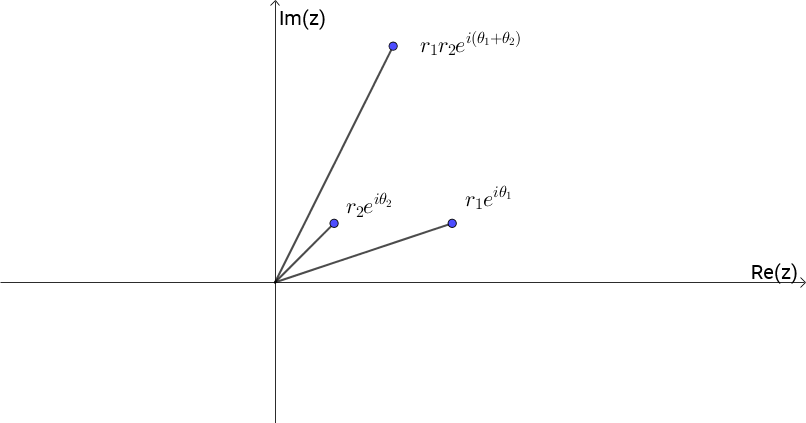
\includegraphics[width=.9\linewidth]{./img/polaer_multi.png}
\caption{\label{polaer_multi}Produktet af to komplekse tal. I dette tilfælde er både \(r_1\) og \(r_2\) større end 1.}
\end{figure}

Division er lige så simpelt i polær form. Kvotienten mellem \(z_1\) og \(z_2\) er givet ved

\begin{equation}
	\frac{z_1}{z_2} = \frac{r_1 \cdot e^{i\theta_1}}{r_2 \cdot e^{i\theta_2}} = \frac{r_1}{r_2} \cdot e^{i (\theta_1 - \theta_2)} \,.
\end{equation}

Sammenhængene \(\left\lvert \frac{z_1}{z_2} \right\rvert = \frac{|z_1|}{|z_2|}\) og \(arg\left(\frac{z_1}{z_2}\right) =arg(z_1)-arg(z_2)\) ses igen at være opfyldt.

Divisionen mellem to komplekse tal kan ses på figur \ref{polaer_divi}.

\begin{figure}[htbp]
\centering
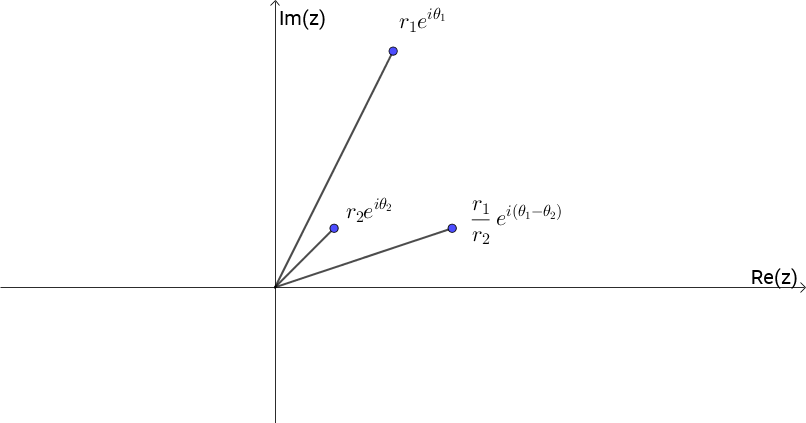
\includegraphics[width=.9\linewidth]{./img/polaer_divi.png}
\caption{\label{polaer_divi}Division af to komplekse tal, hvor \(r_1\) og \(r_2\) begge igen er større end 1.}
\end{figure}

\section{de Moivres formel}
\label{sec:orgdb026a7}

De Moivres formel er en meget vigtig formel. Den knytter komplekse tal sammen med trigonometrien. Den eftervises let ved at sammensætte potenssammenhængen

$$\left(e^{i\theta}\right)^n = e^{i n \theta}$$

med Eulers ligning (\ref{euler})

$$e^{i\theta} = \cos(\theta) + i \sin(\theta)$$

til 

\begin{align}
\left(\cos(\theta) + i \sin(\theta)\right)^n &= \cos(n\theta) + i \sin(n\theta)\,,  
\end{align}

hvor identiteten

$$e^{i n \theta}=\cos(n\theta) + i \sin(n\theta)$$ 

følger af samme Taylor-udvikling som i ligning (\ref{taylor}).

De Moivres formel gælder for alle \(n\) uanset om \(n\) er et reelt, imaginært eller komplekst tal. 

Der er mange anvendelser af de Moivres formel, særligt inden for beregninger med komplekse tal. De følgende 3 afsnit vil vise brugen af de Moivres formel til bevis af trigonometriske identiteter, bestemmelse af enhedsrødder og løsning af polynomiske ligninger med komplekse rødder.

\subsection{Trigonometriske identiteter}
\label{sec:org53281b8}

Den bedste måde, at vise brugen af de Moivres formel til at finde trigonometriske identiteter, illustreres bedst med et eksempel.

\subsubsection*{\emph{Eksempel}}
\label{sec:org1c74004}
\emph{Udtryk \(\cos (3 \theta)\) og \(\sin (3 \theta )\) ved hjælp af potenser af \(\cos(\theta)\) og \(\sin(\theta)\).}

de Moivres formel benyttes

\begin{align}
    \cos (3 \theta) + i \sin(3 \theta) &= \left( \cos(\theta) + i \sin(\theta) \right)^3 \nonumber\\
                    &= \left( \cos^3(\theta) - 3 \cos(\theta)\cdot \sin^2(\theta) \right) + i\left( 3 \sin(\theta) \cdot \cos^2(\theta) -\sin^3(\theta) \right)\,.
\end{align}

De reelle og imaginære dele på hver side af lighedstegnet sættes lig hinanden hver for sig

\begin{align}
\label{cos3}
    \cos(3 \theta) &= \cos^3(\theta) - 3 \cos(\theta) \cdot \sin^2(\theta) \nonumber\\
                   &= \cos(\theta) \left( \cos^2(\theta) -3 \sin^2(\theta)\right)
\end{align}

Parentesen i ligning (\ref{cos3}) kan reduceres ved hjælp af trigonometriens grundrelation

\begin{align*}
    \cos^2(\theta) + \sin^2(\theta) &= 1 \to \\
    \cos^2(\theta) - 1 &= -\sin^2(\theta) \to \\
    3\cos^2(\theta) - 3 &= -3\sin^2(\theta)\,.
\end{align*}

Det sidste udtryk indsættes i ligning (\ref{cos3}).

\begin{align}
    \cos(3 \theta) &= \cos(\theta) \left( \cos^2(\theta) +3 \cos^2(\theta) -3 \right) \to \nonumber \\
    \cos(3 \theta) &= \cos(\theta) \left( 4 \cos^2(\theta) -3 \right) \to \nonumber \\
    \cos(3 \theta) &= 4 \cos^3(\theta) -3\cos(\theta) 
\end{align}

På tilsvarende vis kan \(\sin(3\theta)\) omskrives

\begin{align}
    \sin(3\theta) &= 3 \sin(\theta) \cdot \cos^2(\theta) -\sin^3(\theta) \to \nonumber \\
    \sin(3\theta) &= 3\sin(\theta) - 4\sin^3(\theta) \,. \quad \triangle
\end{align}

Denne metode kan bruges til at finde potensudtryk for \(\sin(n\theta)\) og \(\cos(n\theta)\) for vilkårlige positive heltalsværdier for \(n\).

Den omvendte proces benytter sig af følgende egenskaber for \(z=e^{i\theta}\)

\begin{align}
    z^n + \frac{1}{z^n} &= 2 \cos (n \theta) \label{cosn}\\
    z^n - \frac{1}{z^n} &= 2i \sin (n \theta)\label{sinn} 
\end{align}

Disse egenskaber fremkommer på simpel vis ved brug af de Moivres formel

\begin{align*}
    z^n + \frac{1}{z^n} &=(\cos(\theta)+i \sin(\theta))^n+(\cos(\theta)+i \sin(\theta))^{-n} \to \\
    z^n + \frac{1}{z^n} &=\cos(n\theta)+i \sin(n\theta)+\cos(-n\theta)+i \sin(-n\theta) 
\end{align*}

Herfra udnyttes det at \(\cos(-n\theta) = \cos(n\theta)\) og \(\sin(-n\theta)=-\sin(n\theta)\),

\begin{align}
    z^n + \frac{1}{z^n} &=\cos(n\theta)+i \sin(n\theta)+\cos(n\theta)-i \sin(n\theta) \to \nonumber \\
    z^n + \frac{1}{z^n} &= 2\cos(n\theta)\nonumber\\
    e^{i n \theta} + e^{-i n \theta} &= 2\cos(n\theta).
\end{align}

Udledningen for udtrykket med sinus er som følger

\begin{align}
    z^n - \frac{1}{z^n} &=(\cos(\theta)+i \sin(\theta))^n-(\cos(\theta)+i \sin(\theta))^{-n} \to \nonumber\\
    z^n - \frac{1}{z^n} &=\cos(n\theta)+i \sin(n\theta)-\cos(-n\theta)-i \sin(-n\theta) \to \nonumber\\
    z^n - \frac{1}{z^n} &=\cos(n\theta)+i \sin(n\theta)-\cos(n\theta)+i \sin(n\theta) \to \nonumber\\
    z^n - \frac{1}{z^n} &= 2i \sin(n\theta) \nonumber\\
    e^{i n \theta} - e^{-i n \theta} &= 2i \sin(n\theta)\,. 
\end{align}

I det særlige tilfælde, hvor \(n=1\), gælder

\begin{align}
    z + \frac{1}{z} &= e^{i\theta} + e^{-i\theta} = 2 \cos(\theta) \,, \label{cos2}\\
    z - \frac{1}{z} &= e^{i\theta} - e^{-i\theta} = 2 i \sin(\theta) \,. 
\end{align}

\subsubsection*{\emph{Eksempel}}
\label{sec:org6fdc627}
\emph{Omskriv \(\cos^3(\theta)\) udtrykt ved \(\cos(3 \theta)\) og \(\cos(\theta)\).}

Benytter ligning \eqref{cos2}

\begin{align*}
    \cos^3(\theta) &= \left(\frac{z+\frac{1}{z}}{2}\right)^3 \\
    \cos^3(\theta) &= \frac{1}{2^3} \left(z+\frac{1}{z}\right)^3 \\
    \cos^3(\theta) &= \frac{1}{8} \left(z^3 + 3z + \frac{3}{z}+\frac{1}{z^3}\right) \\
    \cos^3(\theta) &= \frac{1}{8} \left(z^3 + \frac{1}{z^3}\right) +\frac{3}{8} \left(z + \frac{1}{z}\right)\,.
\end{align*}

Den sidste ligning kan omskrives ved hjælp af ligningerne \eqref{cosn} og \eqref{cos2},

\begin{align*}
    \cos^3 (\theta) &= \frac{1}{8}\left(2\cos(3\theta)\right) + \frac{3}{8}\left(2\cos(\theta)\right) \\
    \cos^3 (\theta) &= \frac{1}{4}\cos(3\theta) + \frac{3}{4}\cos(\theta)\,. \quad \triangle
\end{align*}

Dette resultat viser sig, at være en simpel omskrivning af ligningen fra det forrige eksempel. I tilfælde, hvor der bruges større værdier for \(n\), er det generelt bedst at benytte denne direkte metode.


\subsection{Bestemmelse af enhedsrødder}
\label{sec:orgd5f563d}

Ligningen \(z^2=1\) har de velkendte løsninger \(z=\pm1\). Med indførelsen af komplekse tal er det nu muligt at løse den generelle ligning 

$$z^n = 1\,.$$ 

Algebraens fundamentalsætning siger stadig, at ligningen skal have \(n\) løsninger. For at kunne fortsætte omskrives ligningen til

$$z^n = e^{2ik\pi} \,,$$

hvor \(k\) er et heltal. Nu uddrages den n'te rod på hver side af lighedstegnet

$$\sqrt[n]{z^{n}} = \sqrt[n]{e^{2 i k \pi}}= e^{\frac{2 i k \pi}{n}}\,,$$

således at

$$z=e^{\frac{2 i k \pi}{n}}\,.$$

Herved ses det, at løsningerne til \(z^n =1\) er givet ved

$$z_{1,2,\dots,n} = 1, e^{\frac{2 i \pi}{n}},\dots , e^{\frac{2 i (n-1)}{n}} \,,$$

svarende til værdier for \(k\) givet ved \(k=0,1,2,\dots,n-1\). Større heltalsværdier for \(k\) giver ingen nye resultater, da rødderne, som allerede er udregnet, gentages cyklisk for \(k=n,n+1,n+2, \text{etc}\).

\subsubsection*{\emph{Eksempel}}
\label{sec:org59e4e86}
\emph{Bestem rødderne til ligningen \(z^3=1\).}

Benytter den føromtalte metode

$$z = e^{\frac{2 i k \pi}{3}} \,.$$

Der er derfor tre rødder

\begin{align*}
    z_1 &= e^{\frac{2 i \pi \cdot 0}{3}} = e^{0i} = 1 & &\text{ for } k=0\\ 
    z_2 &= e^{\frac{2 i \pi \cdot 1}{3}} = e^{\frac{2 i \pi}{3}} & &\text{ for } k=1\\ 
    z_3 &= e^{\frac{2 i \pi \cdot 2}{3}} = e^{\frac{4 i \pi}{3}} & &\text{ for } k=2 
\end{align*}

Ved indsættelse af \(k=3\) for at beregne \(z_4\) fås:

$$z_4 = e^{\frac{2 i \pi \cdot 3}{3}} = e^{\frac{6 i \pi}{3}} = e^{2 i \pi} = 1 =z_1 \,.$$

Dette viser, at der kun er 3 adskillelige løsninger. Ganske som forventet. \(\triangle\)

Da det gælder at \(\left\lvert z^3\right\rvert = |z|^3\), er det ikke overraskende, at alle enhedsrødderne har modulus på 1, således at de alle ligger på en cirkel med radius 1 i Argand-diagrammet. De tre enhedsrødder fra eksemplet kan ses på figur \ref{enhedsroedder}.

\begin{figure}[htbp]
\centering
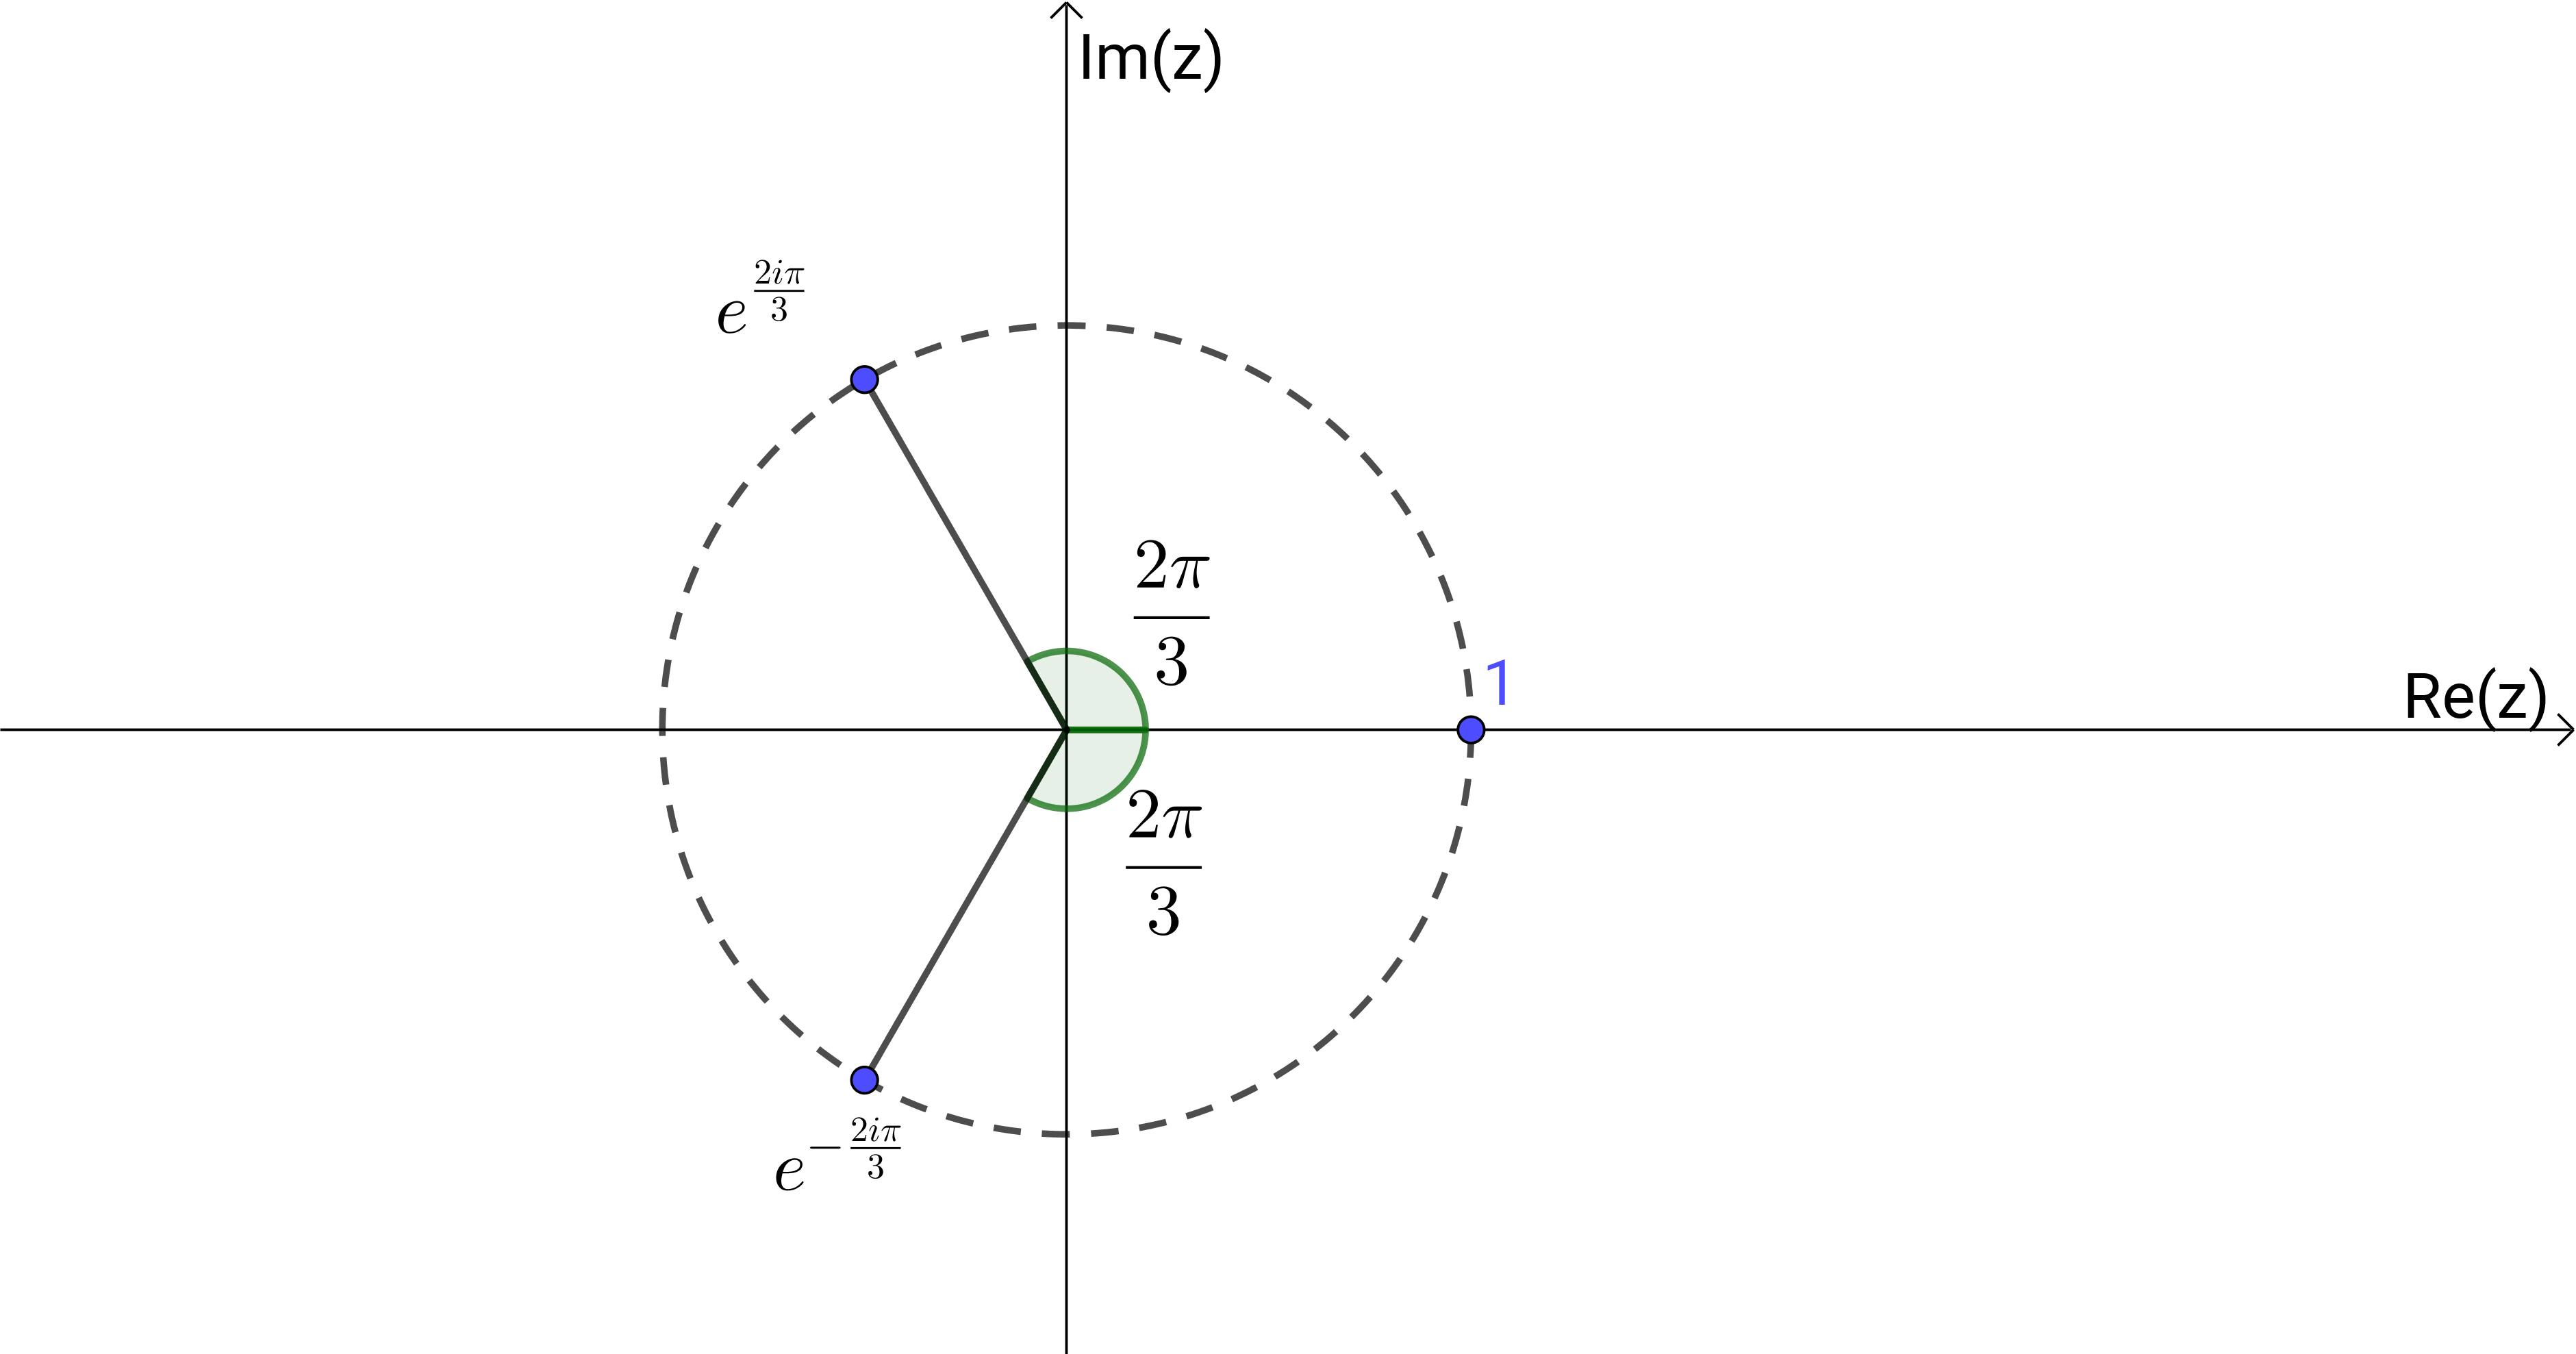
\includegraphics[width=.9\linewidth]{./img/enhedsroedder.png}
\caption{\label{enhedsroedder}De tre enhedsrødder, som er løsningerne til \(z^3=1\), indtegnet i et Argand-diagram.}
\end{figure}

Som en sidste bemærkning om enhedsrødder kan det nævnes, at de tre kubiske enhedsrødder ofte skrives som henholdsvis \(1\), \(\omega\) og \(\omega^2\). Egenskaberne \(\omega^3=1\) og \(1+\omega+\omega^2 =0\) er simple at bevise.

\subsection{Løsning af polynomiske ligninger}
\label{sec:org74254a3}

En tredje anvendelsesmulighed for de Moivres formel er løsning af polynomiske ligninger. Strategien er i første omgang at løse de komplekse polynomiske ligninger for \(z\), som hvis der skulle findes rødder for en reel polynomisk ligning. Efterfølgende kan de komplekse rødder bestemmes.

\subsubsection*{\emph{Eksempel}}
\label{sec:orgcee8e77}
\emph{Løs ligningen \(z^6-z^5+4z^4-6z^3+2z^2-8z+8=0\).}

I første omgang faktoriseres ligningen til

$$\left(z^3-2\right) \left(z^2+4\right) \left(z-1\right) =0 \,.$$

Af denne ligning kan det ses, at \(z^3=2\), \(z^2=-4\) og \(z=1\).

\(z^2=-4\) kan løses simpelt

\begin{align*}
    z^2 &= -4 \to \\
    z &= \pm \sqrt{-4} \\
    z &= \pm \sqrt{-1 \cdot 4} \\
    z &= \pm \sqrt{-1} \cdot \sqrt{4} \\
    z &= \pm i \cdot 2
\end{align*}

\(z^3 =2\) kan løses på tilsvarende måde, som for bestemmelse af enhedsrødder

\begin{align*}
    z^3 &=2 =2 \cdot e^{2 i k \pi} \, ,
\end{align*}

hvor \(k\) er et vilkårligt heltal. Nu uddrages den 3. rod

\begin{align*}
    z = \left(2\right)^{\frac{1}{3}} \cdot e^{\frac{2 i k \pi}{3}} \,.
\end{align*}

Fra forrige afsnit kendes allerede metoden til at finde disse løsninger på nær den faktor \(2^\frac{1}{3}\), som står foran. Det giver da

\begin{align*}
    z_1 &= 2^{\frac{1}{3}} \cdot 1 \quad &\text{ for } k&=0 \\
    z_2 &= 2^{\frac{1}{3}} \cdot e^{\frac{2 i \pi}{3}} \quad &\text{ for } k&=1\\
    z_3 &= 2^{\frac{1}{3}} \cdot e^{-\frac{2 i \pi}{3}} \quad &\text{ for } k&=-1
\end{align*}

For at omskrive \(z_2\) og \(z_3\) til rektangulær form (komponentform, \(z=x+iy\)) benyttes at \(x=\cos(\theta)\) og \(y=\sin(\theta)\),

\begin{align*}
    x_2 &= \cos\left(\frac{2 \pi}{3}\right) = - \frac{1}{2} \\
    y_2 &= \sin\left(\frac{2 \pi}{3}\right) = \frac{\sqrt{3}}{2} \\
    x_3 &= \cos\left(-\frac{2 \pi}{3}\right) = - \frac{1}{2} \\
    y_3 &= \sin\left(-\frac{2 \pi}{3}\right) = - \frac{\sqrt{3}}{2} \,.
\end{align*}

\(z_2\) og \(z_3\) kan da skrives som

\begin{align*}
    z_2 &= 2^{\frac{1}{3}} \left( -\frac{1}{2} + \frac{\sqrt{3}}{2} i \right) \\
    z_3 &= 2^{\frac{1}{3}} \left( -\frac{1}{2} - \frac{\sqrt{3}}{2} i \right) 
\end{align*}

Alt i alt er der da 6 løsninger til ligningen

\begin{align*}
    z_1 &= 2^{\frac{1}{3}} \\
    z_2 &= 2^{\frac{1}{3}} \left( -\frac{1}{2} + \frac{\sqrt{3}}{2} i \right) \\
    z_3 &= 2^{\frac{1}{3}} \left( -\frac{1}{2} - \frac{\sqrt{3}}{2} i \right) \\
    z_4 &= + 2 i \\
    z_5 &= - 2 i \\
    z_6 &= 1 \,.
\end{align*}

Som forventet kan det ses, at der er lige så mange løsninger, som den højeste potens i ligningen. I dette tilfælde altså 6. \(\triangle\)

Et brugbart resultat er, at rødderne i et polynomium med reelle koefficienter optræder i konjugerede par. Dette betyder, at hvis \(z_1\) er en rod, så er \(z^*_1\) også en løsning. Dette kan bevises på følgende måde. 

Tag udgangspunkt i den polynomiske ligning med reelle rødder \(a_0, a_1,\dots,a_n\), hvor \(z\) er en rod

$$a_n z^n + a_{n-1} z^{n-1} + \dots + a_1 z +a_0 =0\,.$$

Nu kompleks konjugeres ligningen

$$a_n^* (z^*)^n + a^*_{n-1} (z^*)^{n-1} + \dots + a^*_1 z^* +a^*_0 =0\,.$$

Da koefficienterne er reelle er \(a_i = a_i^*\) for alle \(i\) fra \(0\) til \(n\). Dermed er forrige ligning lig denne

$$a_n (z^*)^n + a_{n-1} (z^*)^{n-1} + \dots + a_1 z^* +a_0 =0\,.$$

Af dette kan det ses, at \(z^*\) også er en rod til den oprindelige polynomiske ligning.

\section{Komplekse logaritmer og eksponenter}
\label{sec:org0f94610}

Konceptet med en kompleks eksponentialfunktion er allerede blevet introduceret i et tidligere afsnit, hvor det var antaget, at definitionen for eksponentialfunktionen som en Taylorudvikling holdt for både reelle og komplekse tal. På tilsvarende vis kan den komplekse logaritme defineres, og der kan anvendes komplekse eksponenter.

Lad den naturlige logaritme til et komplekst tal \(z\) være givet ved \(w=Ln (z)\), hvor notationen \(Ln\) vil blive forklaret senere. \(w\) skal opfylde

$$z = e^w\,.$$

Ved at benytte ligning (\ref{ee}) ses det, at

$$z_1\cdot z_2 = e^{w_1} \cdot e^{w_2} = e^{w_1 + w_2}\,,$$

Logaritmen på begge sider af lighedstegnet uddrages,

\begin{align}
\label{Ln}
Ln (z_1 \cdot z_2 ) = w_1 + w_2 = Ln (z_1) + Ln (z_2)\,,
\end{align}

hvilket viser, at den velkendte regel for logaritmen af produkter også gælder for komplekse tal. 

Ligning (\ref{Ln}) bruges til yderligere undersøgelse af egenskaberne for \(Ln (z)\). Det er allerede blevet nævnt, at argumentet af et komplekst tal har flere værdier, altså \(arg(z) = \theta + 2 n \pi\), hvor \(n\) er et heltal. Et komplekst tal på polær form skal da i princippet skrives som

$$z= r \cdot e^{i(\theta + 2 n \pi)}\,.$$

Uddragelse af logaritmen på begge sider af lighedstegnet og brug af ligning (\ref{Ln}) giver da

\begin{align}
\label{Ln2}
    Ln (z) = Ln \left(r \cdot e^{i(\theta + 2 n \pi)} \right) = ln(r) + i(\theta + 2 n \pi)\,, 
\end{align}

hvor \(ln(r)\) er den almindelige naturlige logaritme for det reelle positive tal \(r\), og skrives derfor normalt. Fra ligning (\ref{Ln2}) ses det, at \(Ln(z)\) i sig selv har flere værdier. For at undgå flertydighed i værdien, indføres en anden funktion \(ln(z)\), kaldet den \textbf{principielle værdi} af \(Ln(z)\). Denne fås ved at begrænse argumentet af \(z\) til at ligge i intervallet \(-\pi < \theta \leq \pi\).

\subsubsection*{\emph{Eksempel}}
\label{sec:org12a8652}
\emph{Beregn \(Ln(-i)\).}

\(-i\) omskrives til en kompleks eksponent, \(-i = e^{i \left(-\frac{\pi}{2} + 2 n \pi\right)}\).

$$Ln(-i) = Ln \left(e^{i \left(-\frac{\pi}{2} + 2 n \pi\right)}\right) = i\left(-\frac{\pi}{2} + 2 n \pi\right)\,,$$

hvor \(n\) er et heltal. Af dette ses at \(Ln(-i) =-\frac{i \pi}{2}\, , \frac{3 i \pi}{2} \, , \dots\).
Den principielle værdi til \(Ln(-i)\) er da \(ln(-i) = -\frac{i \pi}{2}\). \(\triangle\)


Hvis både \(z\) og \(t\) er komplekse tal, er \(t\) opløftet i \(z\) defineret som

\begin{equation}
\label{tz}
    t^z = e^{z \cdot Ln(t)}\,.
\end{equation}

Da \(Ln(z)\) i sig selv har flere værdier, så har denne definition det også.

\subsubsection*{\emph{Eksempel}}
\label{sec:org2332136}
\emph{Reducer udtrykket \(z=i^{-2i}\).}

Først uddrages logaritmen på begge sider af lighedstegnet.

$$Ln(z) = Ln\left(i^{-2i}\right) = Ln \left(e^{-2i \cdot Ln(i)}\right) = -2i \cdot Ln(i)\,.$$

Den modsatte proces giver

$$e^{Ln(z)} = z = e^{-2i \cdot Ln(i)} \,.$$

\(i\) kan skrives som \(i=e^{i \left( \frac{\pi}{2} + 2 n \pi\right)}\), hvor \(n\) er et heltal, og derfor kan \(Ln(i)\) skrives som

$$Ln(i) = Ln \left(e^{i\left(\frac{\pi}{2} + 2 n \pi\right)}\right) = i \left(\frac{\pi}{2} + 2 n \pi\right).$$

\(z\) kan nu reduceres til

$$z = i^{-2 i} = e^{- 2 i \cdot i \left( \frac{\pi}{2} + 2 n \pi \right)} = e^{2\left( \frac{\pi}{2} + 2 n \pi \right)} = e^{\pi + 4 n \pi}\,,  $$ 

hvilket i sig selv er interessant, da det er en ren reel størrelse fremfor en kompleks. \(\triangle\)

\section{Anvendelse i differential- og integralregning}
\label{sec:org1b7a07b}

Differentiation af trigonometriske funktioner kan i visse tilfælde gøres simplere ved at anvende den polære repræsentation af komplekse tal sammen med de Moivres formel.

\subsubsection*{\emph{Eksempel}}
\label{sec:orgf619e0a}
\emph{Bestem \(\frac{d}{d x} \left( e^{3x} \cdot \cos(4x) \right)\).}

Udtrykket kan differentieres direkte ved hjælp af produktreglen samt kædereglen(reglen for sammensatte funktioner), hvilket dog kan gøres simplere med udnyttelse af komplekse tal. I første omgang betragtes det komplekse tal

$$z= e^{3x} \cdot \left(\cos(4x)+ i \sin(4x)\right) = e^{3x} \cdot e^{4ix} = e^{(3+i4)\cdot x} \,,$$

hvor den trigonometriske funktion er blevet omskrevet til en kompleks eksponentialfunktion. Den reelle del af dette udtryk svarer til det oprindelige udtryk. Nu er det simplere at udføre differentiationen

\begin{align*}
    \frac{d z}{d x} &= (3+i4) e^{(3+i4)\cdot x} \\
                    &= (3+i4) e^{3x}(\cos(4x) + i \sin(4x))\\
                    &= 3 e^{3x} \cos(4x) -4 e^{3x} \sin(4x) +i 3 e^{3x} \sin(4x) + i 4 e^{3x} \cos(4x)\,,
\end{align*}

hvor de Moivre formel igen er brugt til at skrive det komplekse udtryk op på komponentform (rektangulær form). Ved at sætte lighedstegn mellem henholdsvis de reelle og imaginære dele fås, at 

\begin{align*}
\frac{d}{d x} \left( e^{3x} \cos(4x)\right) = e^{3x} \left(3 \cos(4x) -4 \sin(4x)\right)\\
\frac{d}{d x} \left( e^{3x} \sin(4x)\right) = e^{3x} \left(4 \cos(4x) +3 \sin(4x)\right)
\end{align*}

Som det kan ses, er differentiationen gjort simplere og i tilgift fås det sidste differentiale. \(\triangle\)

Komplekse tal kan også udnyttes på nogenlunde tilsvarende vis ved integration af trigonometriske funktioner og eksponentialfunktioner.

\subsubsection*{\emph{Eksempel}}
\label{sec:org073fe82}
\emph{Udfør integralet \(I=\int e^{ax} \cdot \cos(bx) \,dx\).}

Integranden kan betragtes som den reelle del af det komplekse tal

$$e^{ax} \left(\cos(bx) + i \sin(bx)\right) =e^{ax} e^{ibx} = e^{(a+ib)x}\,$$

hvor de Moivres formel er benyttet til at omskrive de trigonometriske funktioner til en kompleks eksponentialfunktion. Integrationen kan nu udføres

\begin{align*}
    \int e^{(a+ib)x} \,dx &= \frac{e^{(a+ib)x}}{a+ib} + c \\
        &= \frac{(a-ib)e^{(a+ib)x}}{(a-ib)(a+ib)} + c\\
        &= \frac{e^{ax}}{a^2+b^2} \left(a e^{ibx} - i b e^{ibx} \right) + c\,.
\end{align*}

Integrationskonstanten er generelt et komplekst tal ( \(c \in \mathbb{C}\) ) og kan skrives som \(c=c_1 + i c_2\), hvor \(c_1, c_2 \in \mathbb{R}\). Dette, sammen med anvendelsen af de Moivres formel, giver

\begin{align*}
    \int e^{(a+ib)x} \,dx &= \frac{e^{ax}}{a^2+b^2} \left(a e^{ibx} - i b e^{ibx} \right) + c \to\\
     \int e^{(a+ib)x} \,dx &= \frac{e^{ax}}{a^2+b^2} \left(a \left(\cos(bx) + i \sin(bx)\right) - i b \left(\cos(bx) + i\sin(bx)\right) \right) + c_1 + i c_2 \\
     \int e^{(a+ib)x} \,dx &= \frac{e^{ax}}{a^2+b^2} \left(a \cos(bx) + b \sin(bx) + i a \sin(bx) - i b \cos(bx)  \right) + c_1 + i c_2 
 \end{align*}

Ved at sætte de reelle og imaginære dele lig hinanden, hver for sig, fås

\begin{align*}
    \int e^{ax} \cdot \cos(bx) \,dx &= \frac{e^{ax}}{a^2+b^2} \left( a \cos(bx) + b \sin(bx)\right) + c_1 \quad \text{ Den reelle del.} \\
    \int e^{ax} \cdot \sin(bx) \,dx &= \frac{e^{ax}}{a^2+b^2} \left( a \sin(bx) - b \cos(bx)\right) + c_2 \quad \text{ Den imaginære del.}
\end{align*}

\hfill \(\triangle\)

\newpage

\section{Opgaver}
\label{sec:org1456264}
\subsection*{Opgave 1}
\label{sec:org95f72bd}
Der er givet følgende fire komplekse tal
$$z=5+2i \quad u = 2+3i \quad v = -1 + 3i \quad 1+i$$

Udregn og reducér i hånden
\begin{enumerate}
\item \(z+u\)
\item \(u-v\)
\item \(u \cdot v\)
\item \(z \cdot u - v\)
\item \(w^2\)
\end{enumerate}
\subsection*{Opgave xx}
\label{sec:org9861ab1}
Udfør multiplikation af følgende komplekse tal:

\begin{enumerate}
\item \(z=1 +2i \quad u=3 + 4i \qquad z\cdot u =?\)
\item \(z=5 +6i \quad u=7 + 8i \qquad z\cdot u =?\)
\item \(z=-3 +2i \quad u=-1 -i \qquad z\cdot u =?\)
\item \(z=4 -2i \quad u=i \qquad z\cdot u =?\)
\end{enumerate}


\subsection*{Opgave xx}
\label{sec:orgb6d491b}
Bestem modulus og argument for hhv. \(z\), \(u\) og \(z \cdot u\).

\begin{enumerate}
\item \(z=1 +2i \quad u=3 + 4i \qquad z\cdot u =-5 + 10i\)
\item \(z=5 +6i \quad u=7 + 8i \qquad z\cdot u =-13 +82i\)
\item \(z=-3 +2i \quad u=-1 -i \qquad z\cdot u = 5 +i\)
\item \(z=4 -2i \quad u=i \qquad z\cdot u =2 + 4i\)
\end{enumerate}


\subsection{Opgave xx}
\label{sec:org6a8e3ac}
Udregn og reducér følgende brøker i hånden, så resultatet kommer til at stå på formen \(z=x+yi\).

\begin{align*}
a &=\frac{-9+2i}{1+2i} \\
b &=\frac{1+i}{1-i} \\
c &= \frac{(1-i)\cdot (1+3i)}{2+i}
\end{align*}

\subsection{Opgave xx}
\label{sec:orgb3a2878}
Beregn modulus og argument for  tæller, nævner og resultat for brøkerne
\begin{align*}
a &=\frac{-9+2i}{1+2i} =-1 + 4i  \\
b &=\frac{1+i}{1-i} = i  \\
c &= \frac{(1-i)\cdot (1+3i)}{2+i} = 2
\end{align*}
\subsection*{Opgave 1}
\label{sec:org480cdac}
Ruten for et orienteringsløb, hvis strækninger er opløst i retlinjede komposanter, kan beskrives med komplekse tal.

Start er placeret i \(0+0i\), og der løbes fra Start til 7 poster, \(P_1-P_7\). Hvis posterne skal nås i den påtænkte sekvens, skal løberne løbe de komplekse strækninger i den herunder viste rækkefølge. Posternes positioner findes ved addition af de komplekse strækninger.

\begin{itemize}
\item Til \(P_1\): \(300\)
\item Til \(P_2\): \(100 + 100i\)
\item Til \(P_3\): \(200i-400\)
\item Til \(P_4\): \(300 + 200i\)
\item Til \(P_5\): \(-200 - 400i\)
\item Til \(P_6\): \(200i - 300\)
\item Til \(P_7\): \(200 - 400i\)
\end{itemize}


\begin{enumerate}
\item Beregn de komplekse talværdier til de 7 punkter på ruten.
\item \(P_7\), som er Mål for orienteringsløbet, er beliggende i nærheden af Start. Hvor stor er afstanden mellem Mål og Start?
\item Hvis \textbf{nord} er i den reelle akses positive retning, hvilken retning skal du da gå i for at komme fra \(P_7\) til \(P_1\)?
\item Hvor langt er løbet planlagt til at være, når der regnes med længdeenheden én meter?
\end{enumerate}
\subsection*{Opgave 2}
\label{sec:org77d15c0}
Betragt de to komplekse tal \(z=3+4i\) og \(w=2-i\). Beregn og indtegn følgende sammenhænge i et Argand-diagram

\begin{enumerate}
\item \(z+w\)
\item \(w-z\)
\item \(w \cdot z\)
\item \(\frac{z}{w}\)
\item \(z^* \cdot w + w^*\cdot z\)
\item \(w^2\)
\end{enumerate}

\subsection*{Opgave 3}
\label{sec:org15b9ebb}
Evaluér eller simplificer følgende udtryk

\begin{enumerate}
\item \(Re\left(e^{2 i z}\right)\)
\item \(\left(-1 + \sqrt{3} \cdot i\right)^{\frac{1}{2}}\)
\item \(\left \lvert e^{\left(i^\frac{1}{2}\right)}\right\rvert\)
\item \(e^{i^3}\)
\item \(Im\left(2^{i+3}\right)\)
\item \(z=1^i\)
\item \(z=i^i\)
\end{enumerate}
\subsection*{Opgave 4}
\label{sec:orgda36f5b}
Ifølge algebraens fundamentalsætning har ethvert polynomium af n'te grad n rødder. I de følgende opgaver ved I da, hvor mange rødder til hvert polynomium, I skal bestemme. I vil blive øvet i forskellige løsningsstrategier i de forskellige opgaver.

\begin{enumerate}
\item \(z^3+z^2-2z =0\)
\item \(z^3-2z^2+2z =0\)
\item \(z^4 =16\)
\item \(z^3+8=0\)
\item \(z^3=27i\)
\end{enumerate}
\subsection*{Opgave 5}
\label{sec:orgc81090c}
Skitsér de dele af Argand-diagrammet hvor følgende udsagn gælder

\begin{enumerate}
\item \(|z| = 2\)
\item \(|z| < 1\)
\item \(1<|z|<2\)
\end{enumerate}

\subsection*{Opgave 6}
\label{sec:org50f6406}
\begin{enumerate}
\item Benyt de Moivres formel med \(n=4\) til at bevise at
\end{enumerate}

$$\cos(4 \theta) = 8\cos^4(\theta) - 8 \cos^2(\theta) +1$$

\begin{enumerate}
\setcounter{enumi}{1}
\item og udled at
\end{enumerate}

$$\cos\left(\frac{\pi}{8}\right) = \left(\frac{2 + \sqrt{2}}{4}\right)^{\frac{1}{2}}\,.$$

\subsection*{Opgave 7}
\label{sec:org430dcf4}
\begin{enumerate}
\item Udtryk \(\sin^4(\theta)\) kun ved hjælp af trigonometriske funktioner med multiplum af vinkler (læs \(\sin(n\theta)\) eller \(\cos(n\theta)\)).

\item Eftervis at den gennemsnitslige værdi over en periode er \(\frac{3}{8}\).
\end{enumerate}


\newpage

\section{Hints og facitliste}
\label{sec:orgd4fd7e5}

\subsection*{Opgave 1}
\label{sec:orgb48bd86}
\begin{enumerate}
\item Positionen af de 7 punkter
\begin{align*}
P_1 &= 300 \\
P_2 &= 400 + 100i \\
P_3 &= 300i \\
P_4 &= 300 + 500i \\
P_5 &= 100 + 100i \\
P_6 &= -200 + 300i \\
P_7 &= -100i
\end{align*}
\item \(\left| P_7 P_0 \right| = 100\)
\item Man skal gå i en retning af \(18.43^{\circ}=0.32\,rad\) i positiv omløbsretning.
\item Løbets samlede længde er:
\begin{align*}
\left| P_0 P_1 \right| &= 300 \\
\left| P_1 P_2 \right| &= 141.42 \\
\left| P_2 P_3 \right| &= 447.21 \\
\left| P_3 P_4 \right| &= 360.56 \\
\left| P_4 P_5 \right| &= 447.21 \\
\left| P_5 P_6 \right| &= 360.56 \\ 
\left| P_6 P_7 \right| &= 447.21 \\
\text{I alt} &= 2504.17 
\end{align*}
\end{enumerate}

\subsection*{Opgave 2}
\label{sec:orgc69665f}
\begin{enumerate}
\item \(5+3i\)
\item \(-1-5i\)
\item \(10+5i\)
\item \(\frac{2}{5} +\frac{11}{5} i\)
\item \(4\)
\item \(3-4i\)
\end{enumerate}


\subsection*{Opgave 3}
\label{sec:org09c1647}
\begin{enumerate}
\item \(e^{-2y} \cos(2x)\)
\item \(\sqrt{2}\cdot e^{\frac{\pi}{3} i}\) eller \(\sqrt{2}\cdot e^{\frac{4 \pi}{3} i}\)
\item \(e^{\frac{1}{\sqrt{2}}}\) eller \(e^{-\frac{1}{\sqrt{2}}}\)
\item \(0.540 - 0.841 i\)
\item \(8 \sin\left(\ln(2)\right) =5.11\)
\item \(z=1\)
\item \(z=e^{-\frac{1}{2} \pi - 2 \pi \cdot n}\)
\end{enumerate}

\subsection*{Opgave 4}
\label{sec:orga51ca8f}
\begin{enumerate}
\item \(z_1=-2\), \(z_2=1+\sqrt{3} i\), \(z_3 = 1- \sqrt{3}i\)
\item \(z_1=2\), \(z_2= 2i\) , \(z_3 = -2\) , \(z_4 =-2i\)
\item \(z_1=\frac{3}{2} \left(\sqrt{3} + i\right)\) ,\(z_2=\frac{3}{2} \left(-\sqrt{3} + i\right)\) , \(z_3 = -3i\)
\item \(z_1=0\), \(z_2=1\) , \(z_3=-2\)
\item \(z_1=0\), \(z_2 =1+i\) , \(z_3=1-i\)
\end{enumerate}

\subsection*{Opgave 5}
\label{sec:orga1e5de1}
Der er tale om koncentriske cirkler.

\subsection*{Opgave 6}
\label{sec:org7ec5883}
\begin{enumerate}
\item Benyt først de Moivres formel. Benyt senere trigonometriens grundrelation.
\item Indsæt \(\frac{\pi}{8}\) på \(\theta\)'s plads. Der kommer til at opstå en skjult andengradsligning, som kan løses.
\end{enumerate}

\subsection*{Opgave 7}
\label{sec:org678b93e}
\begin{enumerate}
\item Svaret er \(\sin^4(\theta) = \frac{1}{8} \cos(4 \theta) -\frac{1}{2} \cos(2 \theta) + \frac{3}{8}\).

Benyt ligning \eqref{cosn} og \eqref{sinn}.

\item Integrér udtrykket fra 0 til \(2\pi\) og divider med \(2 \pi\).
\end{enumerate}


\newpage
\section{Geogebra og komplekse tal}
\label{sec:org1fa965a}

Geogebra har følgende funktioner i sin CAS-del, som gælder for komplekse tal:

\begin{itemize}
\item \(i\) indtastes ved at trykke alt+i.
\item \(e\) indtastes ved at trykke alt+e.
\item \texttt{konjugerede(x)} angiver den kompleks konjugerede til et kompleks tal.
\item \texttt{real(x)} beregner den reelle del af et komplekst tal.
\item \texttt{imaginary(x)} beregner den imaginære del af et komplekst tal.
\item \texttt{TilKompleks(x)} angiver et komplekst tal på komponentform (rektangulær form , \(z=x+iy\)).
\item \texttt{TilPolær(x)} angiver et komplekst tal som (modulus ; argument).
\item \texttt{TilExponentiel(x)} angiver et komplekst tal som \(r \cdot e^{i\theta}\).
\item \texttt{CBeregn(<ligning>,<variabel>)} angiver komplekse løsninger til ligninger.
\item \texttt{CLøsninger(<ligning>,<variabel>)} angiver komplekse løsninger til ligninger.
\end{itemize}

I geogebra kan komplekse tal plottes på flere forskellige måder. I Inputfeltet kan der for eksempel skrives følgende:

\begin{itemize}
\item \texttt{1+2i} - angiver det komplekse tal på komponentform(rektangulær form).
\item \texttt{(3;4*\textbackslash{}pi/3)} - angiver det komplekse tal ud fra modulus og argument. Læg mærke til `;` .

\item \texttt{2*e\textasciicircum{}(-i*pi/4)} - angiver det komplekse tal på eksponentiel form.
\end{itemize}

De tre forskellige komplekse tal kan ses på figur \ref{ggb}.

\begin{figure}[htbp]
\centering
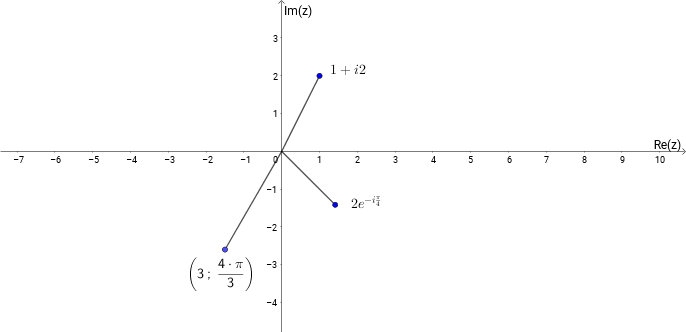
\includegraphics[width=.9\linewidth]{./img/komplekse_tal_ggb.png}
\caption{\label{ggb}Tre forskellige måder at angive komplekse tal på i geogebra.}
\end{figure}
\end{document}